\documentclass[a4paper,11pt]{book}
%\documentclass[a4paper,twoside,11pt,titlepage]{book}
\usepackage{listings}
\usepackage[utf8]{inputenc}
\usepackage[spanish]{babel}
\usepackage{float}
\usepackage{amsmath}
\usepackage{algorithm}
\usepackage[noend]{algpseudocode}
\makeatletter
\def\BState{\State\hskip-\ALG@thistlm}
\makeatother

% \usepackage[style=list, number=none]{glossary} %
%\usepackage{titlesec}
%\usepackage{pailatino}

\decimalpoint
\usepackage{dcolumn}
\newcolumntype{.}{D{.}{\esperiod}{-1}}
\makeatletter
\addto\shorthandsspanish{\let\esperiod\es@period@code}
\makeatother


%\usepackage[chapter]{algorithm}
\RequirePackage{verbatim}
%\RequirePackage[Glenn]{fncychap}
\usepackage{fancyhdr}
\usepackage{graphicx}
\usepackage{afterpage}

\usepackage{longtable}

\usepackage[pdfborder={000}]{hyperref} %referencia

% ********************************************************************
% Re-usable information
% ********************************************************************
\newcommand{\myTitle}{Árboles de clasificación monotónica sobre flujos de datos.}
\newcommand{\myTitleEng}{Monotonic classification trees on data streams.}
\newcommand{\myDegree}{Máster DATCOM: Ciencia de Datos}
\newcommand{\myName}{Carlos Manuel Sequí Sánchez}
\newcommand{\myProf}{Salvador García López}
\newcommand{\myFaculty}{Escuela Técnica Superior de Ingenierías Informática y de
Telecomunicación}
\newcommand{\myFacultyShort}{E.T.S. de Ingenierías Informática y de
Telecomunicación}
\newcommand{\myDepartment}{Departamento de Ciencias de la Computación e I.A.}
\newcommand{\myUni}{\protect{Universidad de Granada}}
\newcommand{\myLocation}{Granada}
\newcommand{\myTime}{\today}
\newcommand{\myVersion}{Version 0.1}

\hypersetup{
pdfauthor = {\myName (email (en) ugr (punto) es)},
pdftitle = {\myTitle},
pdfsubject = {},
pdfkeywords = {Monotonic, data streams, decision tree, Hoeffding tree, classification, MOA},
pdfcreator = {LaTeX con el paquete ....},
pdfproducer = {pdflatex}
}

%\hyphenation{}


%\usepackage{doxygen/doxygen}
%\usepackage{pdfpages}
\usepackage{url}
\usepackage{colortbl,longtable}
\usepackage[stable]{footmisc}
%\usepackage{index}

%\makeindex
%\usepackage[style=long, cols=2,border=plain,toc=true,number=none]{glossary}
% \makeglossary

% Definición de comandos que me son tiles:
%\renewcommand{\indexname}{Índice alfabético}
%\renewcommand{\glossaryname}{Glosario}

\pagestyle{fancy}
\fancyhf{}
\fancyhead[LO]{\leftmark}
\fancyhead[RE]{\rightmark}
\fancyhead[RO,LE]{\textbf{\thepage}}
\renewcommand{\chaptermark}[1]{\markboth{\textbf{#1}}{}}
\renewcommand{\sectionmark}[1]{\markright{\textbf{\thesection. #1}}}

\setlength{\headheight}{1.5\headheight}

\newcommand{\HRule}{\rule{\linewidth}{0.5mm}}
%Definimos los tipos teorema, ejemplo y definición podremos usar estos tipos
%simplemente poniendo \begin{teorema} \end{teorema} ...
\newtheorem{teorema}{Teorema}[chapter]
\newtheorem{ejemplo}{Ejemplo}[chapter]
\newtheorem{definicion}{Definición}[chapter]

\definecolor{gray97}{gray}{.97}
\definecolor{gray75}{gray}{.75}
\definecolor{gray45}{gray}{.45}
\definecolor{gray30}{gray}{.94}

\lstset{ frame=Ltb,
     framerule=0.5pt,
     aboveskip=0.5cm,
     framextopmargin=3pt,
     framexbottommargin=3pt,
     framexleftmargin=0.1cm,
     framesep=0pt,
     rulesep=.4pt,
     backgroundcolor=\color{gray97},
     rulesepcolor=\color{black},
     %
     stringstyle=\ttfamily,
     showstringspaces = false,
     basicstyle=\scriptsize\ttfamily,
     commentstyle=\color{gray45},
     keywordstyle=\bfseries,
     %
     numbers=left,
     numbersep=6pt,
     numberstyle=\tiny,
     numberfirstline = false,
     breaklines=true,
   }
 
% minimizar fragmentado de listados
\lstnewenvironment{listing}[1][]
   {\lstset{#1}\pagebreak[0]}{\pagebreak[0]}

\lstdefinestyle{CodigoC}
   {
	basicstyle=\scriptsize,
	frame=single,
	language=C,
	numbers=left
   }
\lstdefinestyle{CodigoC++}
   {
	basicstyle=\small,
	frame=single,
	backgroundcolor=\color{gray30},
	language=C++,
	numbers=left
   }

 
\lstdefinestyle{Consola}
   {basicstyle=\scriptsize\bf\ttfamily,
    backgroundcolor=\color{gray30},
    frame=single,
    numbers=none
   }


\newcommand{\bigrule}{\titlerule[0.5mm]}


%Para conseguir que en las páginas en blanco no ponga cabecerass
\makeatletter
\def\clearpage{%
  \ifvmode
    \ifnum \@dbltopnum =\m@ne
      \ifdim \pagetotal <\topskip
        \hbox{}
      \fi
    \fi
  \fi
  \newpage
  \thispagestyle{empty}
  \write\m@ne{}
  \vbox{}
  \penalty -\@Mi
}
\makeatother

\usepackage{pdfpages}
\begin{document}
\begin{titlepage}
 
\newlength{\centeroffset}
\setlength{\centeroffset}{-0.5\oddsidemargin}
\addtolength{\centeroffset}{0.5\evensidemargin}
\thispagestyle{empty}

\noindent\hspace*{\centeroffset}\begin{minipage}{\textwidth}

\centering

\includegraphics[width=0.9\textwidth]{imagenes/logo_ugr.jpg}\\[1cm]

\textsc{ \Large TRABAJO FIN DE MÁSTER\\[0.2cm]}
\textsc{ \myDegree}\\[1cm]
% Upper part of the page
% 
% Title
{\Huge \bfseries \myTitle \\
}
\noindent\rule[-1ex]{\textwidth}{3pt}\\[3.5ex]
\end{minipage}

\vspace{1cm}
\noindent\hspace*{\centeroffset}\begin{minipage}{\textwidth}
\centering

\textbf{Autor}\\ {\myName (alumno)}\\[2.5ex]
\textbf{Directores}\\ {\myProf (tutor)}\\[3.5ex]

\includegraphics[width=0.3\textwidth]{imagenes/etsiit_logo.png}\\[0.5cm]
\textsc{Escuela Técnica Superior de Ingenierías Informática y de Telecomunicación}\\
\textsc{---}\\
Granada, septiembre de 2019
\end{minipage}
%\addtolength{\textwidth}{\centeroffset}
%\vspace{\stretch{2}}
\end{titlepage}



\chapter*{}
%\thispagestyle{empty}
%\cleardoublepage

%\thispagestyle{empty}

\begin{titlepage}
 
 
\setlength{\centeroffset}{-0.5\oddsidemargin}
\addtolength{\centeroffset}{0.5\evensidemargin}
\thispagestyle{empty}

\noindent\hspace*{\centeroffset}\begin{minipage}{\textwidth}

\centering

\includegraphics[width=0.9\textwidth]{imagenes/logo_ugr.jpg}

%\textsc{ \Large PROYECTO FIN DE CARRERA\\[0.2cm]}
%\textsc{ INGENIERÍA EN INFORMÁTICA}\\[1cm]
% Upper part of the page
% 

 \vspace{2.5cm}


% Title

{\Huge\bfseries \myTitle\\
}
\noindent\rule[-1ex]{\textwidth}{3pt}\\[3.5ex]
\end{minipage}

\vspace{1.5cm}
\noindent\hspace*{\centeroffset}\begin{minipage}{\textwidth}
\centering

\textbf{Autor}\\ {\myName}\\[2.5ex]
\textbf{Directores}\\
{\myProf }\\[1.5cm]

\includegraphics[width=1\textwidth]{imagenes/decsai}\\[0.1cm]
\textsc{\myDepartment}\\
%\textsc{---}\\
%Granada, mes de 201
\end{minipage}
%\addtolength{\textwidth}{\centeroffset}
\vspace{\stretch{2}}

 
\end{titlepage}






\cleardoublepage
\thispagestyle{empty}

\begin{center}
{\large\bfseries \myTitle}\\
\end{center}
\begin{center}
\myName(alumno)\\
\end{center}

%\vspace{0.7cm}
\noindent{\textbf{Palabras clave}: Monotonic, data streams, decision tree, Hoeffding tree, classification, MOA}\\

\vspace{0.7cm}
\noindent{\textbf{Resumen}}\\

En la presente documentación se tratarán diversas temáticas relativas a la ciencia de datos tales como son, los árboles de decisión, los flujos de datos y la clasificación monotónica.\\

 En la primera parte del documento se pondrá al lector en el contexto del problema mediante la explicación de manera detallada de estas técnicas, así como ejemplos de uso, ventajas e inconvenientes, etc.\\
 
  Posteriormente se procederá a la exposición de la propuesta con el fin de hacer entender al lector que consiste en una técnica novedosa en la materia. Esta consiste en una adaptación a un algoritmo existente de árboles de decisión para flujos de datos que además, en este caso, posean restricciones monotónicas para hacer que los modelos aprendidos a partir de los datos sean más fieles a la realidad.\\
  
 Tras la definición de la propuesta se describirán los detalles de los experimentos implementados para la realización de la propuesta, es decir, el \textbf{marco de trabajo}, el cual incluye una descripción de los conjuntos de datos empleados y medidas para la comparativa de algoritmos, \textbf{resultados} de los experimentos y, finalmente, \textbf{análisis} de estos.

Finalmente se finalizará el documento con una serie de conclusiones y posibles trabajos futuros.

\cleardoublepage


\thispagestyle{empty}


\begin{center}
{\large\bfseries \myTitleEng}\\
\end{center}
\begin{center}
\myName (student)\\
\end{center}

%\vspace{0.7cm}
\noindent{\textbf{Keywords}: Monotonic, data streams, decision tree, Hoeffding tree, classification, MOA}\\

\vspace{0.7cm}
\noindent{\textbf{Abstract}}\\

This documentation will cover various topics related to data science such as decision trees, data flows and monotonic classification.

In the first part of the document the reader will be placed in the context of the problem by explaining in detail these techniques, as well as examples of use, advantages and disadvantages, etc. \\

Subsequently, the proposal will be presented in order to make the reader understand that it consists of a new technique in the field. This consists of an adaptation to an existing decision tree algorithm for data flows that also, in this case, have monotonic restrictions to make the models learned from the data more faithful to reality. \\

After defining the proposal, the details of the experiments implemented for the realization of the proposal will be described, that is, the \textbf{framework}, which includes a description of the data sets used and measures for the comparison of algorithms, \textbf{results} of the experiments and, finally, \textbf{analysis} of these.

Finally, the document will be finished with a series of conclusions and possible future work.

\chapter*{}
\thispagestyle{empty}

\noindent\rule[-1ex]{\textwidth}{2pt}\\[4.5ex]

Yo, \textbf{\myName}, alumno de la titulación \myDegree de la \textbf{\myFaculty}, con DNI 20486926K, autorizo la
ubicación de la siguiente copia de mi Trabajo Fin de Máster en la biblioteca del centro para que pueda ser
consultada por las personas que lo deseen.

\vspace{6cm}

\noindent Fdo: \myName

\vspace{2cm}

\begin{flushright}
Granada a 1 de septiembre de 2019.
\end{flushright}


\chapter*{}
\thispagestyle{empty}

\noindent\rule[-1ex]{\textwidth}{2pt}\\[4.5ex]

D. \textbf{\myProf (tutor1)}, Profesor del Departamento de Ciencias de la Computación e I.A. de la Universidad de Granada.

\vspace{0.5cm}

\textbf{Informa:}

\vspace{0.5cm}

Que el presente trabajo, titulado \textit{\textbf{\myTitle}},
ha sido realizado bajo su supervisión por \textbf{\myName}, y autoriza la defensa de dicho trabajo ante el tribunal que corresponda.

\vspace{0.5cm}

Y para que conste, expide y firma el presente informe en Granada a 1 de Septiembre de 2019 .

\vspace{1cm}

\textbf{El director:}

\vspace{5cm}

\noindent \textbf{\myProf}

\chapter*{Agradecimientos}
\thispagestyle{empty}

       \vspace{1cm}

Llegado a este punto, agradezco la paciencia e interés puesto en mi aprendizaje a todos los profesores que han formado parte, durante todo este año, de poner en mis manos la semilla de conocimiento que me servirá para lanzarme al mundo profesional, así como a mi tutor Salvador García López, quien se ha encargado de ayudarme y supervisar este TFG.
Agradezco a toda mi familia y, con mayor énfasis a mis padres y a mi hermano, el interés y el apoyo que me han ofrecido desde el primer momento, aunque no entiendan del todo las ''letras raras'' en la pantalla de mi ordenador cuando trabajo, o que no nos enseñen a ''hackear'' cosas. Por último, agradezco el haber prolongado el contacto en el ámbito académico con los amigos que hice durante el grado, con buena compañía todo ha sido más sencillo, ya sabéis.

\frontmatter
\tableofcontents
\listoffigures
%
\mainmatter
\setlength{\parskip}{5pt}

%Introduccion del Trabajo Fin de Máster
\chapter[Capítulo 1. Introducción y objetivos]{Introducción y objetivos}

\section{Introducción}

¿Qué es lo primero que se nos viene a la cabeza cuando escuchamos la palabra \textbf{informática}?¿Un ordenador?¿Datos de infinidad de temas y tipos almacenados?¿Programas para facilitar el uso de esos datos?¿Internet?\\

Si mezclamos estas ideas que nos surgen de forma repentina al pensar en dicha palabra, podemos extraer una definición apropiada con facilidad. Una de tantas definiciones para ello, es que la informática se trata de la ciencia que se encarga del almacenamiento, procesamiento y transferencia de información en formato digital a través de un sistema físico con capacidades computacionales (hardware). Mediante dicho \textbf{hardware}, podemos crear programas (\textbf{software}) que faciliten la automatización del proceso de almacenamiento, procesamiento y transferencia de información citados.\\
¿Quién no ha utilizado un ordenador en alguna ocasión para jugar a su juego favorito, imprimir un documento, buscar información por Internet o para ver un vídeo en Youtube de su cantante favorito?\\
Todas estas acciones realizadas con un ordenador (por ejemplo) resultan ser obras de personas con conocimientos específicos en informática necesarios para la creación de estos complejos sistemas dedicados al tratamiento de información de una u otra forma distinta.\\

Si nos adentramos un pequeño paso más hacia aspectos técnicos de la informática, podremos hablar del concepto de \textbf{programación} que, a rasgos muy generales, es el proceso mediante el cual una persona (programador) crea una especie de receta con instrucciones (código fuente) que el ordenador deberá seguir paso a paso para la realización de la tarea deseada por el programador y, es de esta manera la forma de la que se crea un programa.\\

Una vez tenemos la forma de crear procesos automáticos para facilitar a las personas el tratamiento de información, surgen a lo largo de la historia de la informática infinidad de aplicaciones con la que explotar estas capacidades computacionales para sacar provecho económico (empresas privadas), moral (sistemas de vigilancia), académico (clases online) y un largo etcétera de ámbitos de aplicación distintos.\\
Es aquí donde introduzco el concepto clave para la descripción del tema a tratar en este proyecto: \textbf{la Ciencia de Datos}, que en términos muy generales, es un campo interdisciplinar que, a través del uso de ciencias como las matemáticas, estadística e informática, se dedica al análisis y procesamiento de datos para la extracción de información útil de conjuntos de datos(Data Mining), toma de decisiones con respecto a dichos análisis(Estadística inferencial), y automatización de dichos procesos de toma de decisiones(Machine Learning).\\

Como podemos imaginar, poseer conocimientos sobre esta ciencia, supone grandes beneficios para, por ejemplo, empresas que tienen en sus dominios ingentes cantidades de datos sobre sus productos o clientes que los consumen, ya que puede aportarle información para la mejora de la calidad de los productos, mejora de servicios para satisfacer a los clientes, conocimientos sobre el tipo de cliente al que se orienta el producto para crear estrategias de marketing...en conclusión, infinidad de aplicaciones que permiten analizar datos, extraer conclusiones y crear programas automáticos de toma de decisión que un ser humano sería incapaz de realizar en tan poco tiempo y de una forma tan efectiva. Ejemplos de uso de esta ciencia son los de Uber, con su sistema de optimización de ruta en las ciudades, o Amazon, con su sistema de recomendación basado en la predicción de necesidades de sus clientes en función de sus historiales de compra.\\

Para la realización de estos procesos de análisis y procesamiento de datos es indispensable la utilización de algoritmos (esas recetas de las que hablábamos antes) y técnicas complejas de estructuración y análisis de los datos que poseemos en bruto recolectados de alguna manera, que faciliten dichas tareas tanto en tiempo de ejecución como en precisión en la toma de decisiones. Una de estas técnicas de aprendizaje a partir de datos son los llamados \textbf{árboles de decisión}, llamados así porque su estructura (similar a la de un árbol al revés con raíz, ramas y hojas) permite a una computadora ''\textbf{aprender}'' conocimientos sobre un conjunto de datos organizado y \textbf{tomar decisión} en base a ese conocimiento adquirido mediante los ejemplos analizados.\\

Los datos tratados por estas astutas técnicas de análisis no siempre permanecen almacenados y ordenados previo análisis, si no que pueden provenir de fuentes que generan ingentes cantidades de datos de forma periódica y sin pausa, los cuales han de ser tratados de forma rápida y constante para poder obtener una buena representación de su comportamiento y poder generar una toma de decisión correcta. Estos son los llamados \textbf{flujos de datos o data streaming}.\\

Es bien sabido también que, toda ayuda que el ser humano pueda poner de su parte para la mejora de los algoritmos de análisis y toma de decisiones, será bien recibida por cualquiera de las técnicas utilizadas en la Ciencia de Datos. Es esta la idea de hacer uso de las llamadas \textbf{restricciones monotónicas} de las cuales hablaremos durante todo el documento. Consiste básicamente en aportar información subyacente a un tipo problema específico para ayudar al algoritmo a alcanzar mejores resultados.

\section{Motivación}

Tras el estudio a lo largo del máster de todo lo detallado en el apartado anterior y tras ver ejemplos y ejemplos de uso de los citados árboles de decisión, técnicas de data streaming y técnicas de uso de restricciones monotónicas, no he sido capaz de encontrar artículos ni ejemplos donde se haga uso de estos tres elementos de forma conjunta con el fin de obtener mejores resultados sobre flujos de datos con capacidades de obedecer restricciones monotónicas mediante el uso de árboles de decisión.\\

Como bien he dicho anteriormente, toda ayuda que el ser humano pueda aportar a los algoritmos que se encargan de la resolución de cualquier problema, será bien recibida, por tanto, pienso que incluir conocimiento mediante restricciones de monotonía sobre los datos a un algoritmo que utiliza árboles de decisión para resolver problemas de data streaming hará que se obtengan mejores resultados.\\\\

De esta manera, la motivación principal es aportar a la comunidad científica un novedoso tratamiento de algoritmos ya existentes para mejorar la calidad de estos en problemas específicos relativos a la Ciencia de Datos.

\section{Objetivos y estructuración de la memoria}


El objetivo incial de este documento es dotar al lector de los conocimientos y el contexto necesarios sobre las distintas técnicas a utilizar para que logre entender la finalidad de la propuesta. En esta primera parte del documento se explicarán en profundidad los elementos ya mencionados a formar parte de objeto de estudio:

\begin{itemize}
	\item Clasificación sobre flujos de datos.
	\item Clasificación con restricciones monotónicas.
	\item Árboles de decisión y su uso con data streams y restricciones monotónicas (por separado, evidentemente).
\end{itemize}


Una vez hayamos dotado al lector de la contextualización del problema, el siguiente objetivo es la descripción detallada de la propuesta con el fin de hacer entender las ideas necesarias para la creación del nuevo algoritmo, los pasos a seguir para lograrlo y los resultados esperados con ello, seguido de la explicación del software utilizado para tal propósito, así como su uso.\\

Finalmente, aparecerá en este documento una exposición de los experimentos realizados con la propuesta, además de comparaciones de sus resultados con los de los algoritmos que citaremos más adelante, con el propósito de observar si la propuesta cumple el cometido de resultar ser mejor en los aspectos que deseemos.\\
Acompañado de estas comparaciones y para finalizar el documento, presentaremos también una serie de conclusiones y trabajos futuros a desarrollar para continuar con esta línea de trabajo.

\newpage


\chapter[Capítulo 2. Background en problemas]{Background en problemas}

\section{Data streaming classification}

Los sistemas tradicionales basados en el uso de memoria, entrenados de una forma fija mediante conjuntos de entrenamiento y los cuales generan modelos estáticos, no están
preparados para procesar los datos altamente detallados disponibles en procesos como, por ejemplo, el continuo análisis de datos generados por los sensores de una máquina que trabaja sin descanso, lo cual crea una gran cantidad de datos que ha de ser procesada de forma rápida con el fin de generar modelos predictivos consistentes
que se adapten a situaciones cambiantes y puedan reaccionar de forma rápida y eficaz a dichos cambios.

El Machine Learning extrae conocimiento en forma de modelos y patrones de unos datos de naturaleza cambiante. Hoy en día la generación de datos, gracias a las capacidades
tecnológicas de las que disfrutamos, se produce a altas velocidades, tanto es así, que se pone, en cuanto a velocidad, por delante del procesamiento de dichos datos, lo cual
quiere decir que generamos datos a mayor velocidad de lo que las capacidades computacionales que tenemos ahora mismo nos permiten procesarlos.\\
Desde este punto de vista, en estos casos conviene modelar los datos como flujos de datos transitorios en lugar de como tablas de datos persistentes.

\begin{figure}[H]
	\centering
	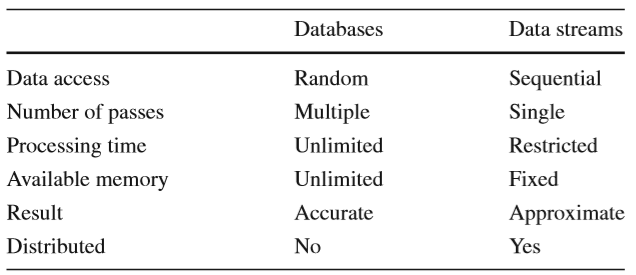
\includegraphics[width=0.9\textwidth]{imagenes/tabla1} 
	\caption{Resumen entre las diferencias principales entre el procesamiento estándar de una base de datos y el procesamiento de flujo de datos. \cite{ref1}}
\end{figure}



\subsection{Tipos de algoritmos para data stream}

Existen dos tipos distintos de algoritmos que trabajan sobre flujos de datos:
\begin{itemize}
	\item \textbf{Insert-only model}: donde los datos entran al sistema de forma secuencial.
	\item \textbf{Insert-delete model}: donde los elementos que entran pueden ser eliminados o actualizados.
\end{itemize}

Desde el punto de vista de los sistemas de control de flujo de datos(DSMS), existen varios problemas que requieren técnicas de procesamiento no exactas para evaluar el flujo continuo de datos que requieren una cantidad ilimitada de memoria.

Estos algoritmos de procesamiento flujos de datos producen soluciones aproximadas dentro de un rango de error admisible para ciertas aplicaciones, con una alta probabilidad, relajando así las restricciones a la hora de obtener una solución exacta.

Los sistemas de control de flujos de datos han desarrollado un conjunto
de técnicas que almacenan resúmenes de datos compactos suficientes para resolver consultas. Estas aproximaciones requieren un equilibrio entre el accuracy y la cantidad de memoria usada para almacenar los resúmenes, con una restricción adicional de tiempo de procesado de los datos.


\subsection{Aproximación y aleatorización}

Dentro del marco del data streaming, como ya hemos dicho, está permitido ofrecer respuestas aproximadas dentro de un pequeño rango de error ($\epsilon$), con una pequeña probabilidad de fallo ($\delta$) para obtener respuestas con una probabilidad de que 1-$\delta$ se encuentre en el intervalo de radio $\epsilon$.

Los algoritmos que usan estas aproximacióon y aleatorización son referidos por dichos ($\epsilon$,$\delta$).\\
la idea consiste básicamente en mapear cada espacio grande de entrada en una sinopsis pequeña.\\
La aproximación y randomización han sido usadas en solventar problemas como minería de reglas de asociación, items frecuentes, k-means...


\subsection{Ventanas de tiempo}

Para la realización del cómputo estadístico referente al modelo de flujos, no nos interesa el total de los datos existentes, si no los más recientes, entendiendo que son los que mejor explican la situación a la que nos enfrentamos y pudiendo, de esta forma, deshacernos de grandes cantidades de datos que no nos son útiles.

Las técnicas más simples para este tipo de tratamiento de datos, utilizan una ventana deslizante de tamaño fijo, con un funcionmiento FIFO (first in fist out).

Definimos dos tipos de ventana deslizante:
\begin{itemize}
	\item \textbf{Basada en secuencia}: donde el tamaño de ventana queda definido por el número de observaciones del data set (tamaño fijo o variable en el tiempo).
	\item \textbf{Basada en marca de tiempo}: donde el tamaño de ventana está definido en términos de duración. Una ventana de este tipo de tamaño t consiste en todos los elementos cuya marca de tiempo
	se situa dentro del intervalo de tiempo t del actual periodo de tiempo.
\end{itemize}

El hecho de monitorizar, analizar y extraer conocimiento de flujos de datos de alta velocidad, puede hacer que existan diversos niveles de \textbf{granularidad} a la hora de 
almacenar los datos. Conforme más antiguos son los datos que disponemos, mayor granularidad requeriremos en la información (es decir, menor precisión). Cuanto más
reciente sean los datos, el grano ha de ser más fino, ya que requerimos más precisión al tratarlos debido a que son más importantes (este es llamado el\textbf{ modelo de ventana de tiempo inclinado}).

\subsubsection{Ejemplo de algoritmo de ventana de tiempo}

\textbf{AdWin-ADaptive sliding WINdow}: mantiene una ventana variable con respecto a los items recientemente vistos con la propiedad de que la ventana tiene un tamaño maximal
estadísticamente consistente con la hipótesis de que no haya habido un cambio en la media del valor dentro de la ventana. Un fragmento viejo de la ventana se desecha
si hay alguna evidencia de que tiene un valor distinto al del resto de la ventana.


\subsection{Sampling}

El sampling (o muestreo) consiste en la selección del subconjunto de datos a analizar en intervalos periódicos, utilizado para calcular estadísticas del flujo (valores esperados).\\
Este tipo de técnicas reduce la cantidad de datos a procesar, por tanto, el coste computacional.\\
Como contra a su uso, podemos decir que pueden ser una fuente de errores, por ejemplo, en aplicaciones dedicadas a la detección de valores extremos o anomalías, ya que, a la hora de realizar el sampling podemos estar eliminando dichas instancias. El problema principal es obtener una muestra representativa.


Técnicas de muestreo:
\begin{itemize}
	\item \textbf{Random sampling}: muestreo aleatorio de los datos (todas las instancias con la misma probabilidad de ser escogidas).
	\item \textbf{Reservoir sampling}: consiste en mantener una muestra de tamaño K de reserva. A medida que fluyen los datos, cada nuevo elemento tiene una probabilidad k/n (donde n son los datos visualizados hasta el momento) de reemplazar un antiguo dato.
	\item \textbf{Load shedding}: elimina secuencias del flujo de datos cuando se producen cuellos de botellas en las capacidades de procesamiento.
\end{itemize}

\subsection{Sinopsis, bocetos y resúmenes}
A continuación describimos tres métodos de compactación de información para la generación de modelos sobre los ya comentados conjuntos de datos reducidos para data streaming:

\begin{itemize}
	\item \textbf{Sinopsis}: estructuras de datos compactas que resumen datos para su posterior consulta.
	\item \textbf{Data sketching}: herramienta de reducción de dimensionalidad. Usa proyecciones aleatorias de datos con cierta dimensión d a un espacio de cierto conjunto de dimensiones.
	\item \textbf{Data stream summary (by Cirnide and Muthukrishnan)}: usado para aproximaciones ($\epsilon$,$\delta$) para resolver consultas de rango, consultas puntuales y consultas innerproduct.
\end{itemize}


\subsection{Algoritmos para el aprendizaje de flujos de datos}

Hulten y Domingos presentan un método general para aprender de bases de datos grandes y arbitrarias.
Este método consiste en derivar un límite superior para la pérdida del learner en función del número de ejemplos usados en cada paso del algoritmo. De esta forma, se minimiza el número de ejemplos requeridos en cada paso del algoritmo, a la vez que se garantiza que el modelo obtenido no difiere de forma significante de aquel que se obtendría con todos los datos.Esta metodologia de datos se ha aplicado de forma exitosa en k-means, clustering jerárquico de variables, árboles de decision, etc.

El aprendizaje de conjuntos de datos grandes puede ser más efectivo con el uso de algoritmos que ponen más énfasis en la gestión del sesgo (bias). Uno de estos algoritmos es el \textbf{Very Fast Decission Tree system (VFDT)}: es un algoritmo de aprendizaje basado en árboles de decisión que ajusta de forma dinámica su sesgo en función
de que haya nuevos ejemplos disponibles.

En la inducción del árbol de decisión, el principal problema consiste en tomar la decisión de cuando expandir el árbol, instalando un test de división y generando nuevas hojas.
La idea básica consiste en usar un conjunto pequeño de ejemplos para seleccionar el test de divisón para colocar en un nodo del arbol de decisión.
Si tras ver un conjunto de ejemplos, la diferencia en resultados entre ambos test de división no satisface un test estadistico (Hoeffding bound), entonces VFDT procede a examinar
más ejemplos.
Esto solo toma una decisión cuando hay evidencias estadísticas suficientes a favor de un test particular.
Esta estrategia satisface la estabilidad del modelo (baja varianza), controla el overfitting, mientras que puede alcanzar un numero acrecentado de grados de libertad (low bias)
incrementando el número de ejemplos.
En VFDT se aprende un árbol de decisión de forma recursiva reemplazando hojas por nodos de decisión. Cada hoja almacena las estadísticas necesarias sobre los valores de los
atributos. Dichas estadísticas necesarias son aquellas que se necesitan por una función de evaluación heurística que realiza el cálculo de el resultado de los test de división 
basada en el valor de los atributos.
Cuando hay un ejemplo disponible, atraviesa el árbol desde la raíz hasta una hoja evaluando el atributo requerido en cada nodo y siguiendo la rama correspondiente al valor
del atributo en el ejemplo.
Cuando el ejemplo llega a una hoja, la estadística de las hojas por las que ha pasado han sido actualizadas.
Entonces cada condición basada en los valores de los atributos ha sido evaluada.
El nuevo nodo de decisión tendrá tantos descendientes como el número de posibles valores tenga el atributo escogido (por lo que el árbol no es necesariamente binario).
Los nodos de decisión tan solo contienen la información sobre el test de división instalado en ellos.
La innovación principal de los VFDT es el uso de los Hoeffding bounds para decidir cuantos ejemplos han de verse previa instalación de un test de decisión en un nodo
hoja.
VFDT ha sido implementado también para tratar con atributos continuos, hojas funcionales y con flujos de datos no estacionarios. 
Una característica interesante de VFDT es que tiene la capacidad de congelar las hojas menos comprometedoras en entornos de trabajo con memoria limitada. Existen  también ejemplos de VFDT con bagging y boosting y para aprender regresión y modelos de árboles.

El CVFDT es una extensión para flujos de datos cambiantes en el tiempo. Este genera árboles de decisión alternativos en nodos donde hay evidencia de que el test de división no
es ya apropiado. El sistema reemplaza el árbol actual con uno nuevo que resulta ser más preciso.


\subsection{Problemas en el aprendizaje sobre data streams}

El objetivo de la minería de datos es la habilidad de mantener de forma permanente un modelo de decisión preciso.
Este problema requiere algoritmos que se adapten a los datos conforme esten disponibles para poder aprender de ellos.
Además, los datos desactualizados han de ser olvidados para dejar de tenerlos en cuenta a la hora de crear el modelo, cosa que ha de ocurir en la presencia de 
información con una distribución no estacionaria presente. El aprendizaje en flujos de datos requiere por tanto algoritmos incrementales de aprendizaje que tengan en
cuenta el llamado "concept drift".

La solución a estos problemas requieren nuevas técnicas de muestreo y randomización, y nuevos algoritmos aproximados, incrementales y decrementales.
Algunas propiedades deseables para algoritmos de flujos de datos:
\begin{itemize}
	\item \textbf{Incrementalidad}
	\item \textbf{Aprendizaje online}
	\item \textbf{Tiempo constante de procesado de cada ejemplo}
	\item \textbf{Un solo escaneo sobre el conjunto de datos de training}
	\item \textbf{Tener en cuenta el concept drift}
\end{itemize}


Los algoritmos de aprendizaje incrementales y decrementales requieren una permanente actualización del modelo de decisión conforme llegan datos nuevos. Esta habilidad 
de actualizar el modelo mediante las propiedades de los nuevos datos es importante, pero no suficiente, ya que también es necesaria la habilidad de olvidar información
anticuada para dar un giro en el aprendizaje realizado, dejando de tener en cuenta los items antiguos: decremental learning.

Evidentemente existe una balanza entre la ganancia en rendimiento ofrecido por el algoritmo y la manutención de la característica de actualización de este, lo que hace que 
el cómputo realizado por el algoritmo sea más complejo. Ante esta balanza, con el fin de no acrecentar el cómputo, haciendo que el algoritmo decida de forma dinámica
qué información borrar y cuál no, surge la ya comentada técnica de ventana deslizante.

De forma general, es complicado asumir que, en el manejo de flujos de datos durante un largo tiempo, estemos tratando con datos acordes a una distribución de probabilidad
estacionaria. En sistemas complejos y en largos periodos de tiempo, debemos esperar cambios en la distribución de los items.

Una aproximación natural para estas tareas incrementales son los algoritmos de aprendizaje adaptativo, algoritmos incrementales que tienen en cuenta el concept drift.
El concept drift en sí, se refiere al cambio de concepto que sufren los datos a la largo del tiempo, cada vez con cierta permanencia mínima.
Hay algoritmos que implementan el olvido de información antigua teniendo en cuenta este cambio de concepto, lo que los hace mucho más precisos que los propios algoritmos
que realizan la eliminación de información en forma de tamaño de ventana prefijado.\\
Con el uso de los algoritmos de detección de concept drift podemos averiguar cuando y por qué ha cambiado el comportamiento del flujo de datos.\\
Estos algoritmos no poseen la información de mundo cerrado de la que disponen los algoritmos convencionales para el tratamiento de datos estáticos, si no que han de ser
capaces de adaptarse a un mundo abierto cambiante de datos para diferenciar entre cambio de concepto y ruido en los datos.

A la hora de evaluar los resultados en el contexto de los flujos de datos, es interesante tener en cuenta la evolución del acierto de nuestro algoritmo a lo largo del tiempo
con los cambios de concepto acaecidos.





















\section{Ordinal and monotonic classification}

Comenzamos este apartado definiendo primeramente un par de conceptos básicos para adentrarnos de forma correcta en el significado
de la clasificacción ordinal y monotónica:

\begin{itemize}
	\item \textbf{Principio de dominancia}: a mayor valor en atributos de una instancia, mayor sera el
	valor de la clase a la que se asigna dicha instancia.
	Usando el termino de ''relación de dominancia'' decimos que una instancia x domina a
	otra instancia x' cuando cada una de las variables de entrada de x (atributos de x)
	son mayores o iguales que cada uno de los de x', se denota x$>$=x' y por tanto
	x tendra asignada una etiqueta de clase mayor que x'.
	\item \textbf{Función monótona}: una función es monótona si x$>$=x' -$>$ h(x)$>$=h(x'). Es decir, si x domina a x', la
	inferencia de clase de x ha de ser superior a la de x'.
\end{itemize}

Una vez definidos estos conceptos, podemos describir el sentido de la clasificación ordinal con restricciones monotónicas así como su diferencia con respecto a la clasificación ordinal simple:

\begin{itemize}
	\item La \textbf{clasificación ordinal con restricciones monotónicas} maneja conocimiento subyacente del
	problema sobre clases ordenadas, atributos ordenados y una relación monotónica entre
	la evaluación de los atributos de una instancia y la asignación de esta a una clase.
	\item Si no hay relación de monotonía en la asociación de una clase a una instancia, 
	pero las clases si poseen un orden, entonces se considera\textbf{ clasificación ordinal} simplemente.
\end{itemize}

Con las restricciones de monotonía presentes se puede trabajar con una amplia
variedad de funciones sin temor a que introduzcan más restricciones que 
la de monotonía: es posible hacer inferencia de la clase sobre todas las funciones
monótonas.\\
La clasificación monotónica puede ser directa (más habitaciones, precio mayor
de una casa), o inversa (más polución, precio menor de la casa).\\
Normalmente en problemas de clasificación monotónica reales, las restricciones
monotónicas son consideradas en un subconjunto de características del dataset, no en todos los atributos.

Ejemplos de uso de monotonicidad:
\begin{itemize}
	\item Comparación de dos compañías donde una domina sobre la otra en términos de
	todos los indicadores financieros. Debido a esto, la compañía dominante
	ha de tener una evaluación final superior a la compañía dominada. Un uso
	de esto, es la predicción de la calificación crediticia usada por los bancos.
	\item House pricing: el precio de una casa será superior cuantas más habitaciones
	posea, mejor sea la calidad del aire acondicionado y menor sea la polución
	en el ambiente.
\end{itemize}



\subsection{Restricciones monotónicas}

La motivación del uso de restricciones monotónicas viene dada por los siguienes aspectos:
\begin{itemize}
	\item El tamaño del espacio de la hipótesis es reducido, lo que facilita el
	proceso de aprendizaje. 
	\item Otras métricas además de la precisión, como la consistencia con respecto
	a estas restricciones, pueden ser usadas por los expertos para aceptar
	o rechazar el modelo. Estas técnicas de evaluación de restricciones
	monotónicas las veremos más adelante con el fin de poder evaluar 
	la consistencia de estas.
\end{itemize}

Las restricciones impuestas a continuación, son restricciones con respecto a la probabilidad de distribución en la generación de 
datos, además de imposiciones sobre la función de perdida bajo las cuales
el clasificador óptimo de Bayes es monótono.

\subsubsection{Dominancia estocástica}

El principio de dominancia no siempre
se aplica en la práctica de forma tan restrictiva, por lo que hemos de 
hablar en términos probabilísticos a la hora de referirnos a dichas
restricciones.

Decimos entonces que, siendo 'k' una de las posibles clases a tomar en el 
dominio por una instancia 'x', y siendo 'y' la etiqueta asignada a dicha
instancia 'x', si la restricción monótona nos dice que x$>$=x', entonces
la dominancia estocástica nos dice que P(y$<$=k|x)$<$=P(y$<$=k|x').
Es decir, que la probabilidad de que el valor asignado (y) a la instancia 
dominante (x) sea mayor que cierto valor fijado de la clase (k), es mayor
que la probabilidad de que el valor asignado (y) a la instancia dominada(x')
sea mayor que ese mismo cierto valor de la clase fijado.

La relación de dominancia estocástica entre distribuciones se denota así:

\begin{figure}[H]
	\centering
	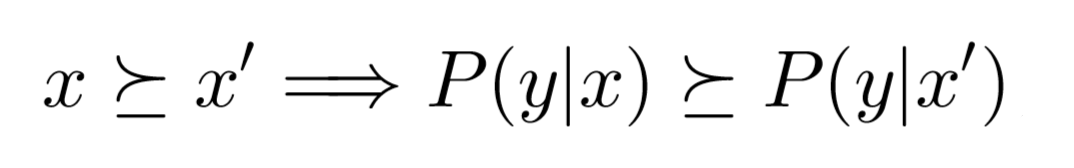
\includegraphics[width=0.4\textwidth]{imagenes/f1}
\end{figure}

Donde P(y$|$x) y P(y$|$x') denotan las distribuciones condicionales de la clase en x y x'. 

\subsubsection{Clasificador monótono de Bayes}

En el problema de clasificación el objetivo es encontrar el clasificador más
parecido al clasificador de Bayes, es decir, esta es nuestra función objetivo.
Sabiendo esto, se convierte en requisito el hecho de que este también aplique
las restricciones de monotonía que hemos enunciado. 

\textbf{Problema}: aunque la
distribución de probabilidad tiene restricciones monotónicas, el clasificador
de Bayes no siempre las mantiene.
Para solucionar este problema y mantener la monotonía en el clasificador de 
Bayes, han de imponerse las siguientes restricciones a la función de perdida
(L):

\begin{itemize}
	\item L(y,k+1)-L(y,k) $>$= L(y+1,k+1)-L(y+1,k) \\
	Esta característica de la función de pérdida es necesaria
	en la clasificación con restricciones monotónicas, si no no
	tendría sentido minimizar el riesgo dentro de la clase de las funciones monótonas.\\
	(Demostrado en \cite{ref2})
	\item La siguiente definición de convexidad es necesaria también para
	mantener la restricción de monotonía en el clasificador de Bayes:
		\begin{itemize}
			\item Siendo L(y,k) = c(y-k) (con c(0)=0)
			\item La función c(k) es convexa si, para todo k entre -(k-1) y (k-1):\\
			c(k) $<$= (c(k-1)+c(k+1))/2
			\item El clasificador de Bayes es monótono si y solo si c(k) (que es
			la V-shaped loss function) es convexa.
		\end{itemize}
\end{itemize}


\subsection{Métodos de clasificación no paramétricos}

Los métodos no paramétricos son así llamados porque explotan la clase de todas las
funciones monótonas. Estos métodos no hacen ninguna asunción más sobre el modelo que la de 
las restricciones monotónicas.

\subsubsection{Aproximación Plug-In}

Pretenden \textbf{estimar la distribución condicional de la clase}. Provienen de la
clasificación isotónica (monótona creciente o decreciente)

Hemos de construir un método para estimar P(y$|$x), sabiendo que P(y$|$x) posee
dos ventajas:
\begin{enumerate}
	\item La distribución condicional permite la determinación de la predicción 
	óptima para cualquier función de pérdida.
	\item La distribución condicional mide la confianza de la predicción.
\end{enumerate}


\textbf{Problema de la clasificación binaria y la regresión isotónica.}

En la aproximación plug-in se propone usar un vector de estimadores de densidad
condicional p = (p1,....,pn), el cual es una regresión isotónica del vector de
etiquetas y = (y1,...,yn). Es decir, p nos da la probabilidad de que x 
pertenezca a cada una de las clases existentes en y.

Dicho vector p es la solución del problema: SUM((yi-pi)\^2) sujeto a las restricciones de
monotonicidad (Xi$>$=Xj -$>$ pi$>$=pj). Por ello p minimiza el error cuadrático en 
el conjunto de los vectores monótonos p=(p1,..,pn) para cada x.

La elección de la función de error (función de perdida de error cuadrático)
parece ser arbitraria. Puede verse que haciendo uso de otras funciones
de perdida, se llega al mismo resultado.

La regresión isotónica es un problema de optimización cuadrática con 
restricciones lineales, por ello puede ser resuelta de forma eficiente con
la mayoría de los resolutores de optimización de propósito general.

\textbf{Problema multiclase.}

Está basado en la regresión isotónica multiclase y, la idea es descomponer el problema de K-clases en varios problemas binarios
y aplicar regresión isotónica a cada uno de los problemas.
Está demostrado que la descomposición del problema de estimación de 
probabilidad para el caso de multiclase, siempre forma una adecuada 
distribución de probabilidad, es decir, que siempre son no negativos
y la suma es igual a 1.


\subsubsection{Aproximación directa}

Consideramos la clasificación directa basada en la\textbf{ minimización del riesgo 
empírico} dentro de la clase de todas las funciones monótonas.\\
Aunque este tipo de funciones no se pueden describir con un número 
finito de parámetros, la minimización del riesgo puede realizarse debido a 
que solo estamos interesados en valores de funciones monótonas en ciertos
puntos, los incluidos en D (training set).

Una función monótona minimizando el riesgo empírico puede obtenerse resolviendo
el siguiente problema de optimización:

\begin{itemize}
	\item Minimizar: SUM(L(yi,di)).
	\item Teniendo en cuenta las restricciones de monotonía.
	\item Donde di son variables del problema (valores de la función monótona óptima
	en puntos de D)
\end{itemize}

El problema puede tener \textbf{otra interpretación} interesante: reetiquetar las
instancias para hacer el dataset monótono de forma que las etiquetas de las
instancias sean lo mas parecidas a las del conjunto original, donde esta 
similitud es medida en términos de la función de pérdida. Estas nuevas
etiquetas serán los nuevos valores óptimos de las variables di. 
Este reetiquetado puede realizarse en el proceso de preprocesamiento
y corresponde a la \textbf{corrección del error no paramétrico}.

Como el problema de clasificación no paramétrica se asimila al de la regresión
isotónica (exceptuando que ahora se considera una salida discreta), será llamado
ahora ''clasificación isotónica'' y su solución optima d\^ será llamada
''clasificación óptima de y''




\newpage


\chapter[Capítulo 3. Background en algoritmos de árboles de decisión]{Background en algoritmos de árboles de decisión}

\section{Fundamentos de árboles de decisión}

 Los \textbf{árboles de decisión} \cite{ref3} son un tipo de algoritmos de aprendizaje supervisado (tanto para clasificación como para regresión) utilizado en diversos ámbitos como la inteligencia artificial, las finanzas, el marketing, etc. \\ Dado un conjunto de datos se fabrican diagramas de construcciones lógicas en forma de ramificaciones de árboles, muy similares a los sistemas de predicción basados en reglas, que sirven para representar y categorizar una serie de condiciones que ocurren de forma sucesiva, para la resolución de un problema.
 
 Adentrándonos en los aspectos más técnicos de este tipo de modelos de predicción, cabe destacar que las variables de entrada y de salida pueden ser tanto categóricas como continuas y que divide el espacio de los predictores (variables independientes) en regiones distintas y no superpuestas, tal como veremos en la siguiente figura.
 
 \begin{figure}[H]
 	\centering
 	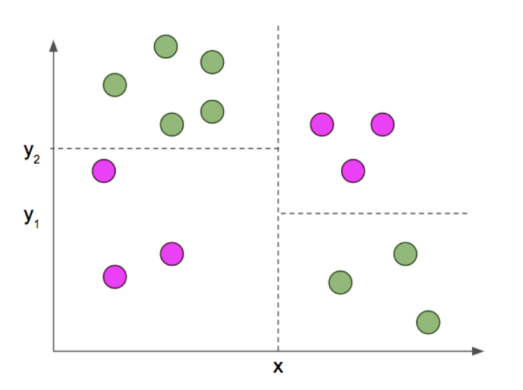
\includegraphics[width=0.7\textwidth]{imagenes/ejemploArboles} 
 	\caption{Ejemplo de árbol de decisión \cite{ref4}}
 \end{figure}
 
 Estas divisiones se realizan creando sobre la población (el conjunto de datos) subconjuntos lo más homogéneos posible entre las muestras que componen un grupo y lo más heterogéneo posible entre los distintos subconjuntos.\\
 Para la efectuación de esta separación, el algoritmo se basa en las variables de entrada más significativas, es decir, las que mejor separan las muestras.
 
 A continuación podemos observar las diferentes partes de un árbol de decisión.
 
  \begin{figure}[H]
 	\centering
 	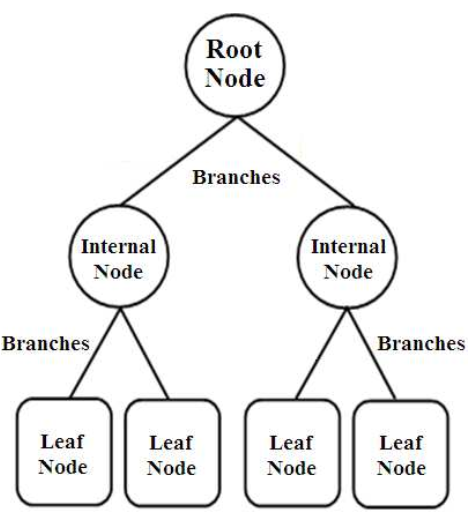
\includegraphics[width=0.5\textwidth]{imagenes/ejemploArbol} 
 	\caption{Partes de un árbol de decisión \cite{ref5}}
 \end{figure}

\subsection{Terminología:}
\begin{itemize}
	\item \textbf{Nodo raíz}: Es el primero de los nodos del árbol y forma la población completa.
	\item \textbf{Ramificación}: Son las ramas que conectan todos los nodos del árbol por donde pasan las muestras para ser clasificadas.
	\item \textbf{Nodo de decisión}: Son aquellos donde las muestras se evalúan para decidir por qué rama continuar el camino hacia la solución.
	\item \textbf{Nodo terminal/hoja}: Estos son los nodos solución, una vez la muestra llega a este tipo de nodo, el proceso de evaluación de esta ya ha finalizado, por lo que habrá sido clasificada en alguno de los grupos categóricos existentes.
	\item \textbf{Poda}: Consiste en cortar u obviar una rama del árbol en la creación de un árbol, basándonos en cierta propiedad escogida, para evitar el recorrido del árbol completo y ahorrar de esta forma costos computacionales, así como para hacer frente al sobreajuste.
	\item \textbf{Rama/subárbol}: Es el conjunto de nodos y ramas completo que queda estrictamente por debajo de un nodo escogido del árbol total.
	\item \textbf{Nodos padre e hijo}: Dado un nodo del árbol, sus nodos hijo son todos aquellos que quedan conectados directamente a él únicamente en el nivel inferior siguiente. De esta forma, esos nodos hijo, comparten ese mismo padre.
\end{itemize}


\subsection{¿Regresión o clasificación?: similitudes y diferencias.}

\subsubsection{Similitudes}

Ya sabemos, por ejemplo, que un árbol de decisión divide el espacio de los predictores en regiones no solapadas mediante el uso de los predictores más significativos.

Los árboles de decisión actúan bajo la llamada \textbf{separación binaria recursiva}, basada en un método greedy el cual decidirá en cada momento cuál será la mejor separación en el instante actual para encontrar el mejor árbol. El término 'binaria' hace alusión al tipo de división acaecido en cada nodo, es decir, que cada nodo divide en dos el espacio de los predictores. El término 'recursiva' se refiere a que el algoritmo realiza este proceso de forma reiterada hasta llegar a un criterio de parada predefinido.

Este proceso nos conduce a la generación de un árbol completo si no hacemos uso de criterios de parada, lo que nos lleva de forma directa al problema del sobreajuste, obteniendo un modelo de una pésima calidad a la hora de evaluar nuevos datos. Por esto mismo es necesario difinir criterios de parada que realicen podas sobre el árbol para generar modelos lo suficientemente genéricos que eviten ese overfitting.

\subsubsection{Diferencias}

Las diferencias entre ambos modelos son bastante evidentes: para conjuntos de datos donde se utiliza una variable dependiente continua, utilizamos árboles de regresión, mientras que cuando la variable dependiente es categórica, usamos árboles de clasificación.\\
Dado esto, el \textbf{valor de los nodos hoja} no pueden ser calculados de la misma forma para ambas técnicas, por lo que, en \textbf{árboles de regresión}, utilizamos la \textbf{media} del valor de salida de las muestras que caen en dicho nodo hoja, mientras que en \textbf{árboles de clasificación} utilizamos la \textbf{moda} para asignar un valor de salida a nuevas muestras.

\subsection{Ventajas e inconvenientes de los árboles de decisión}

\subsubsection{Ventajas}

\begin{itemize}
	\item Fáciles de comprender a la hora de interpretar los resultados.
	\item El tipo de dato utilizado no es una limitación.
	\item Es un método no paramétrico, es decir, en el que no es necesario hacer suposiciones sobre el espacio de distribución y la estructura del clasificador.
	\item Resulta útil a la hora de detectar la relevancia de los predictores aún habiendo una gran cantidad de estos.
	\item No son influidos por outliers ni valores perdidos (hasta cierto punto), por lo que requieren una menor limpieza de datos en comparación con otros métodos.
\end{itemize}

\subsubsection{Inconvenientes}

\begin{itemize}
	\item Producen sobreajuste, por lo que hay que tener cuidado con ello mediante el uso de restricciones y la aplicación de poda.
	\item A la hora de trabajar con variables continuas, el árbol de decisión pierde información en el momento en el que categoriza dichas variables para la generación del árbol.
	\item No son del todo competentes con los mejores algoritmos de aprendizaje supervisado en cuanto a precisión en la predicción, es decir, no resultan ser tan efectivos ensambladores o SVM por ejemplo.
	\item Son sensibles al ruido en los datos, ya que este puede modificar de forma significativa la estructura del árbol.
\end{itemize}

\subsection{Creación del árbol}

Como ya sabemos, un árbol comienza desde un nodo raíz donde se encuentra clasificada toda la población y, conforme vamos profundizando por las ramas inferiores, vamos obteniendo subconjuntos cada vez más y más homogéneos con respecto a la variable de salida.

Para hacer posible esto necesitamos que nuestro modelo tome, por cada nodo, una decisión de separación de los datos basada en la ganancia de pureza (esa homogeneidad en los subconjuntos) al utilizar uno u otro predictor en cada uno de los nodos de decisión para crear esas particiones del espacio sucesivas.\\
Es decir, para cada nodo, se evalúa mediante unos medidores de pureza, cual es el predictor o característica del conjunto de datos en dicho instante que separa de mejor forma los datos que tenemos en ese momento con respecto a la variable de salida. Se escogerá en cada nivel, el predictor que mayor pureza ofrezca al árbol de decisión.

De esta forma vamos construyendo de manera progresiva ramas y más ramas del árbol haciendo uso de una técnica greedy de selección de característica a evaluar en cada nivel del árbol para la toma de decisión a la hora de generar nuevos nodos hijos.

\subsubsection{¿Cómo medimos esa ganancia de homogeneidad?}

Para los\textbf{ árboles de regresión} sabemos que el objetivo de cada decisión del árbol en la creación de nuevas separaciones es minimizar la función RSS (\textbf{Residual Sum of Squares}), una medida de error usada también en la regresión lineal. Es por ello que en cada nodo se escogerá una forma de particionar los datos mediante el uso de un predictor u otro, atendiendo a cuál minimiza en mayor medida dicha fórmula.

\begin{figure}[H]
	\centering
	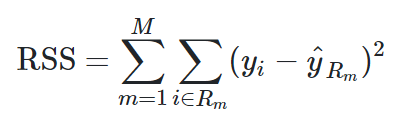
\includegraphics[width=0.5\textwidth]{imagenes/rss} 
	\caption{Recursive Binary Splitting in regression trees \cite{ref6}}
\end{figure}

Como el problema que nos concierne en este caso es el de \textbf{árboles de clasificación}, no entraremos en más detalles acerca de esta fórmula, ya que RSS no puede ser utilizado como criterio de separación binaria en este tipo de árboles.

Una aproximación natural a RSS es el '\textbf{ratio de error en la clasificación}', basado simplemente en la fracción de las observaciones de training en dicha región que no pertenecen a la clase más común de esta. Se calcula de la siguiente forma:

\begin{figure}[H]
	\centering
	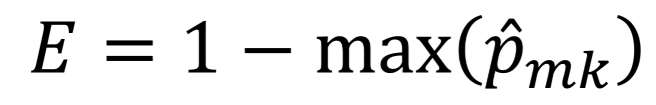
\includegraphics[width=0.5\textwidth]{imagenes/cer} 
	\caption{Recursive Binary Splitting in classification trees (classification error rate) \cite{ref7}}
\end{figure}

Donde $\widehat{P}$mk es la proporción $\widehat{P}$ de las observaciones de train de la región \textbf{m} que pertenecen a la clase \textbf{k}. Por tanto, el máximo de $\widehat{P}$mk hace alusión a la proporción máxima de elementos de train que siguen la moda en dicha partición.\\
Por desgracia esta medida de error no es lo suficientemente sensible conforme el árbol crece, por lo que es preferible el uso de otras medidas como el índice Gini y la Entropía.

Ya sabemos que buscamos nodos con una distribución de clase lo más homogénea posible. Con el fin de medir esa pureza en cada nodo, podremos utilizar los siguientes métodos ya mencionados:
\begin{itemize}
	\item \textbf{Índice GINI}: nos indica como de pura es una región del espacio. En este caso la pureza la definimos como la proporción de items de la región que pertenecen a una misma clase. Si la región contiene un índice
	alto de pureza, entonces el índice Gini será bajo (muy próximo a 0), siguiendo la siguiente fórmula:
	\begin{figure}[H]
		\centering
		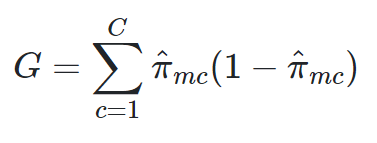
\includegraphics[width=0.5\textwidth]{imagenes/gini} 
		\caption{Recursive Binary Splitting in classification trees (gini) \cite{ref8}}
	\end{figure}
	Donde $\widehat{\pi}$mc nos indica la proporción \textbf{$\widehat{\pi}$} de items pertenecientes a la misma clase \textbf{c} en la región/nodo \textbf{m}.
	\item \textbf{Entropía (E-score)}: Se encarga también de la medida de homogeneidad de un nodo. En este caso, los resultados obtenidos al aplicar la siguiente fórmula a cada nodo para observar el nivel de entropía, quedan más visibles con respecto a la medida Gini (es decir, se ve de forma más clara el nivel de homogeneidad de un nodo). Una entropía = 0 significa homogeneidad total, una entropía = 1 significa homogeneidad nula.
	\begin{figure}[H]
		\centering
		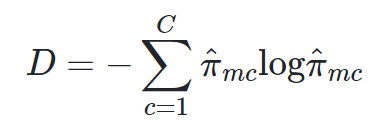
\includegraphics[width=0.5\textwidth]{imagenes/entropia} 
		\caption{Recursive Binary Splitting in classification trees (entropia) \cite{ref8}}
	\end{figure}
\end{itemize}

\subsubsection{¿Cómo evitamos el overfitting?}

Una vez hemos escogido nuestra estrategia de creación del árbol, necesitamos indicarle al algoritmo cuándo ha de terminar de construirlo el uso de restricciones (prepruning) y su posterior poda (postpruning) para evitar de esta forma un sobreajuste a los datos.\\

\textbf{Prepruning: establecimiento de parámetros}
\begin{itemize}
	\item Definir un número de observaciones mínimo sobre un nodo para que sea considerada una ramificación sobre él.
	\item Definir un número mínimo de observaciones sobre un nodo hoja.
	\item Establecer una profundidad vertical máxima para el árbol.
	\item Limitar el número máximo de nodos hoja.
	\item Parar si la expansión del nodo actual no mejora la medida de pureza utilizada actual.
\end{itemize}

\textbf{Proceso de Postpruning}:
\begin{enumerate}
	\item Crear un árbol muy grande con o sin restricciones de prepruning.
	\item Recorrer el árbol de abajo hacia arriba para ir cortando las hojas que nos dan ganancias negativas.
\end{enumerate}

De esta forma podemos mantener ramas que, sin el proceso de postpruning podrían haber sido recortadas, pero que nos llevan a soluciones mejores que las que se ofrecen si este proceso por culpa del uso de la técnica greedy.


\section{Hoeffding Trees y otros algoritmos de data streaming}

Como ya sabemos, los algoritmos dedicados al data streaming han de seguir los siguientes requisitos:
\begin{itemize}
	\item Procesar una muestra en cada momento y hacerlo tan solo una vez.
	\item Usar una cantidad de memoria limitada.
	\item Trabajar en un tiempo limitado.
	\item Estar listo para la predicción en cualquier momento.
\end{itemize}

Además, nuestro algoritmo ha de estar dotado de técnicas de detección de cambios en la distribución de los datos para evitar la disminución de la precisión en la predicción cuando esto suceda.

\subsection{Hoeffding tree (VFDT)}

Un árbol de Hoeffding es un algoritmo de inducción de árbol de decisión incremental capaz de aprender de flujos de datos masivos, suponiendo que la distribución que genera ejemplos es estacionaria, es decir, que no cambia con el tiempo. Los árboles Hoeffding explotan el hecho de que una pequeña muestra a menudo puede ser suficiente para elegir un atributo de división óptimo. Esta idea está respaldada matemáticamente por el Hoeffding bound, que cuantifica el número de observaciones (en nuestro caso, ejemplos) necesarias para estimar algunas estadísticas dentro de una precisión prescrita (en nuestro caso, la bondad de un atributo). \cite{ref9}

Algunas de las técnicas de clasificación para data streaming tienen los siguientes \textbf{problemas}:
\begin{itemize}
	\item Son altamente sensibles a la demanda de ejemplos.
	\item Carecen de alta eficiencia, siendo en algunos casos más lentos que un algoritmo batch.
\end{itemize}

Ante estos problemas se plantea\textbf{ Hoeffding-tree} ya que:
\begin{itemize}
	\item El aprendizaje de un Hoeffding-tree toma un tiempo constante en cada nuevo ejemplo, lo que lo hace adecuado para el aprendizaje de flujos de datos.
	\item Los árboles resultantes son similares a los creados con un batch learner convencional.
\end{itemize}

\subsubsection{Hoeffding bound.}

Hulten y Domingos presentan un método general para aprender de bases de datos grandes y arbitrarias.
Este método consiste en derivar un límite superior para la pérdida del learner en función del número de ejemplos usados en cada paso del algoritmo. De esta forma, se minimiza el número de ejemplos requeridos en cada paso del algoritmo, a la vez que se garantiza que el modelo obtenido no difiere de forma significante de aquel que se obtendría con todos los datos. Esta metodología de datos se ha aplicado de forma exitosa en k-means, clustering jerárquico de variables, árboles de decisión, etc.

Con el fin de cumplir con los requisitos establecidos al principio de este apartado para el tratamiento de flujos de datos, los autores proponen la cota Hoeffding para ser capaces de decidir la cantidad de instancias necesarias a evaluar para alcanzar un cierto nivel de confianza a partir del cual sabemos que no es necesario evaluar más ejemplos para seleccionar un atributo mediante el cual realizar la partición del árbol en el nodo actual.\\
Es decir, una vez alcanzada la cota de Hoeffding, el atributo que seleccionemos para el particionamiento del espacio de predictores, sera el mismo que seleccionaríamos si analizásemos una infinidad de ejemplos con el clasificador (evidentemente, con cierto nivel de confianza).

La idea básica consiste en usar un conjunto pequeño de ejemplos para seleccionar el test de divisón para colocar en un nodo del árbol de decisión.
Si tras ver un conjunto de ejemplos, la diferencia en resultados entre ambos test de división no satisface un test estadístico (Hoeffding bound), entonces VFDT procede a examinar más ejemplos.

En VFDT se aprende un árbol de decisión de forma recursiva reemplazando hojas por nodos de decisión. Cada hoja almacena las estadísticas necesarias sobre los valores de los
atributos. Dichas estadísticas necesarias son aquellas que se necesitan por una función de evaluación heurística que realiza el cálculo del resultado de los test de división 
basada en el valor de los atributos.
Cuando hay un ejemplo disponible, atraviesa el árbol desde la raíz hasta una hoja evaluando el atributo requerido en cada nodo y siguiendo la rama correspondiente al valor
del atributo en el ejemplo.
Cuando el ejemplo llega a una hoja, la estadística de las hojas por las que ha pasado han sido actualizadas.
Entonces cada condición basada en los valores de los atributos ha sido evaluada.

El nuevo nodo de decisión tendrá tantos descendientes como el número de posibles valores tenga el atributo escogido (por lo que el árbol no es necesariamente binario).
Los nodos de decisión tan solo contienen la información sobre el test de división instalado en ellos.

\textbf{Problema}: VFDT no incluye soporte para el concept-drift por lo que, ante cambios en la distribución de los datos, los resultados del algoritmo pueden ser malos.

\textbf{Cálculo de la cota:}

Teniendo n variables independientes $r_{1}...r_{n}$ con un rango R y una media $\bar{r}$, el Hoeffding bound afirma con una probabilidad 1-$\delta$ que la media real es al menos $\bar{r}$-$\epsilon$ donde:
\begin{figure}[H]
	\centering
	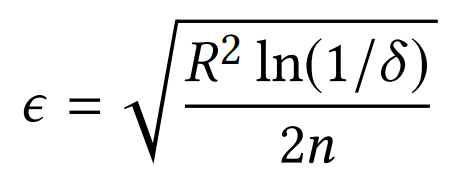
\includegraphics[width=0.3\textwidth]{imagenes/hoeffdingbound} 
	\caption{Cálculo del límite de Hoeffding \cite{ref10}}
\end{figure}

Sabiendo que $\delta$ es la tolerancia al fallo a la hora de escoger un atributo en un nodo dado.\\
Una vez calculado el Hoeffding bound, se realizará la división si sucede una de las siguientes ocurrencias:
\begin{itemize}
	\item La diferencia entre la ganancia ofrecida por el mejor atributo para la división y la ganancia ofrecida por el segundo mejor atributo, es mayor que el Hoeffding bound.
	\item El Hoeffding bound es menor que un parámetro de desempate (tie-breaking) establecido para cuando se dé el caso de que el Hoeffding bound es lo suficientemente pequeño pero los dos mejores atributos escogidos para la división son demasiado similares como para que se cumpla la condición anterior, lo que podría llevar a un estancamiento del árbol. El parámetro de desempate, según la literatura, suele establecerse a un valor de 0.05, que se suele alcanzar con unas 3.400 instancias analizadas.
\end{itemize}

\subsection{Otros algoritmos de data streaming}

Muchas bases de datos grandes presentan cambios en la distribución de los datos conforme avanza la generación de estos, es decir, posee un cambio de concepto en el tiempo, un \textbf{concept drift}. El hecho de que un algoritmo de flujos de datos no esté preparado para esos efectos cambiantes puede producir un empeoramiento de los resultados predictivos con el paso del tiempo, por lo que conviene tenerlo en cuenta a la hora de implementar esta clase de algoritmos.

Ante este problema, surgen técnicas como el uso de una \textbf{ventana deslizante} que tenga en cuenta los X ejemplos más recientes para asegurarnos de aprender siempre un modelo que tenga en cuenta el concepto actual se los datos, olvidando conceptos anteriores. Ante esta situación, ha de tenerse cuidado de escoger un valor adecuado de X, ya que ha de ser lo suficientemente grande como para tener un número suficiente de ejemplos con los que aprender el modelo y lo suficientemente pequeño como para abarcar un solo concepto de los datos.

\subsubsection{CVFDT}

Un algoritmo que utiliza este concepto de ventana deslizante es el llamado\textbf{ Concept-adapting Very Fast Decision Tree (CVFDT)} que, evidentemente, contiene además las características del VFDT. A continuación la explicación de su funcionamiento\cite{ref12}:

\begin{figure}[H]
	\centering
	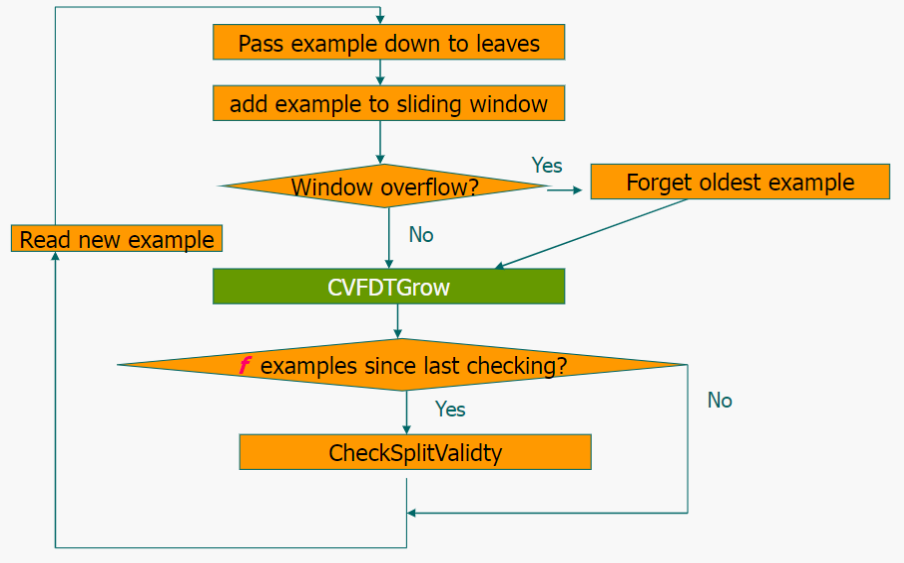
\includegraphics[width=1\textwidth]{imagenes/cvfdt} 
	\caption{Ciclo CVFDT \cite{ref11}}
\end{figure}

\begin{enumerate}
	\item Entra un nuevo ejemplo al ciclo.
	\item Se añade a la ventana deslizante.
	\item Se comprueba si se excede la cantidad de ejemplos necesarios en dicho nodo para poder decidir el atributo apropiado para la división de los nodos hijos. En caso de excederse dicho tamaño de ventana, se elimina el ejemplo más antiguo.
	\item CVFDTGrow: Se incrementan las estadísticas de cada uno de los nodos por los que pasa el ejemplo tanto en el árbol principal como en los subárboles. Si se ha alcanzado la cantidad suficiente de elementos analizados como para expandir un nodo hoja, escogemos el mejor de los atributos para expandir y se procede a ello.
	\item CheckSplitValidity: Comprueba si comenzar un árbol alternativo o no basado en el atributo que mejor realiza la división en cada uno de los nodos. Se realiza una comprobación de las estadísticas de cada nodo observando si se produce un cambio de concepto con el nuevo ejemplo, en cuyo caso es posible que el atributo escogido anteriormente en dicho nodo posea una ganancia menor que otro, por lo que el algoritmo creará un subárbol alternativo cuya raíz será ese atributo que tenga mejor gain que el actual en dicho nodo.
\end{enumerate}

Cada uno de los nodos de decisión ha de tener las estadísticas suficientes para poder olvidar información en caso de que se produzca un cambio de concepto. Para ello, cada uno de los nodos posee un ID monotónicamente incremental que permite al algoritmo validar las decisiones previamente tomadas y realizar el olvido de información inútil en los cambios de concepto. Cuando un ejemplo antiguo es eliminado de la ventana, se recorre el árbol para decrementar las estadísticas por cada uno de los ID de los nodos por los que ha pasado.


\subsubsection{HATT}

Otro algoritmo que implementa una solución más eficiente a la presentada por Hoeffding tree es el \textbf{Hoeffding Anytime Tree} \cite{ref10}, el cual asegura conseguir mejores resultados explotando la información conforme le llega al modelo en lugar de esperar a traspasar el Hoeffding bound y, realizando correcciones sobre estas decisiones de elección de atributo para la división siempre que sea necesario.
Por tanto, en cuanto se detecte una división útil en cualquiera de las hojas del árbol, se realizará de forma inmediata y esta, será reemplazada tan pronto como otra alternativa mejor sea identificada.

Además de esto, algunos experimentos muestran que el algoritmo, aún no habiendo sido tratado para ello, muestra algunas características de tratamiento de concept drift.

\subsubsection{Option trees}

Con el objetivo de introducir a Hoeffding tree mayor estabilidad y romper la barrera que posee VFDT para mirar hacia adelante, surje Option trees\cite{ref13}.\\
Consiste en una estructura que representa a múltiples árboles en lugar de a uno solo como hace VFDT. Una instancia nueva puede bajar por varios caminos del árbol contribuyendo de diferentes maneras en diferentes opciones. La clase de un ejemplo de test se determina por un comité(mayoría de voto o pesos) hecho por las predicciones de todas los nodos hoja alcanzados. El concepto es crear múltiples opciones pero de la misma forma que lo hace Hoeffding tree.\\
Esta nueva representación de un árbol difiere únicamente de la representación hecha para VFDT en que contienen unos nodos llamados \textbf{nodos opción} que se encargarán de evaluar a los ejemplos que pasen por ellos mediante múltiples tests para determinar por qué ramas dejarle pasar.\\
En este nuevo método, un ejemplo que entra al árbol puede influir en varios nodos hoja distinto, mientras que en el Hoeffding tree, un solo ejemplo tan solo puede influir en un solo nodo hoja.

\section{Árboles de decisión monotónicos}

Conociendo las restricciones monotónicas descritas en el anterior capítulo, hemos de ser capaces de extrapolar dichos conocimientos a los árboles de decisión para poder resolver problemas de este estilo.

\textbf{Recordamos} que, siendo X e Y valores de atributos y $C_x$ y $C_y$ las clases asignadas a X e Y respectivamente, se cumple una \textbf{relación de monotonía} entre el par atributo-clase (X,$C_x$) y el par (Y,$C_y$) si y solo si (X,$C_x$) domina a (Y,$C_y$), viceversa o son exactamente iguales (tanto en valores de sus atributos como en clase asignada).

Hacemos uso de \textbf{este conocimiento sobre un árbol de decisión} de la siguiente manera:\\
Siendo (P,$C_p$) y (Q,$C_Q$) dos caminos distintos del mismo árbol de decisión (donde P y Q son atributos y $C_p$ y $C_q$ son nodos respuesta), estos son monotónicos entre sí, si cumplen las mismas reglas de monotonía descritas justo en el párrafo anterior (relación de dominancia).\cite{ref14}

\subsection{Problema:}
Un conjunto de datos donde todos sus ejemplos guardan una relación de monotonía entre sí, no garantiza que genere un árbol de decisión monotónico a través de algoritmos teóricos TDIDT(top-down induction decision tree) que usan la entropía como selector de atributos.

Crear un árbol de decisión que cumpla las restricciones de monotonía estudiadas y que al mismo tiempo vele por la minimización de error (la precisión) no es tarea sencilla. 

\subsection{¿Cómo creamos un árbol de decisión monotónico?}

Aún no siendo una tarea simple, existen \textbf{métodos de creación de estos árboles} como los que describimos a continuación.

\subsubsection{Método basado en matriz}

Uno de estos métodos es el \textbf{basado en matriz}. Teniendo ya construido un árbol con k ramas, construimos una matriz simétrica M de tamaño k x k donde el valor $m_{ij}$ es un 1 en caso de que la rama de la fila i no guarde una relación de monotonía con la rama de la columna j y un 0 en caso contrario. Cada columna (y fila) está asociada con un contador que hace referencia a la suma de los unos que contiene, de esta forma sabemos con qué cantidad de ramas no guarda la relación de monotonía. Comenzamos eliminando (podando) aquellas ramas del árbol que tienen un contador mayor de no-monotonía y actualizando los contadores del resto de ramas hasta llegar a obtener una matriz llena de ceros o hasta llegar a una matriz 1 x 1, en cuyo caso M sería una matriz de no-monotonicidad.

\subsubsection{Método aleatorio}

Otro método más rápido a la hora de ejecutar es tomar inicialmente de forma aleatoria una rama del árbol y declararla como monotónica. A partir de aquí ir tomando siempre de forma aleatoria cada una de las demás ramas del árbol, compararlas con las ramas ya declaradas monotónicas y, o bien descartarlas (en caso de no guardar relación de monotonía con las ya declaradas monotónicas) o bien introducirlas en el conjunto de ramas declaradas monotónicas.

\subsubsection{Método de evaluación de monotonicidad y precisión}

Describimos en este apartado una métrica para que tenga en cuenta tanto el error como las restricciones monotónicas a la hora de decidir si expandir un nodo del árbol de decisión, lo que lo convierte en el tercero de los métodos que describiremos para la creación de árboles de decisión montónicos.

Primeramente definimos una medida de no-monotonicidad para los árboles de decisión:\\
El \textbf{índice de no-monotonicidad} nos dice el ratio entre el número real de pares de ramas no monotónicas de un árbol de decisión y el número máximo de pares que podrían no haber sido monotónicos con respecto a otras en el mismo árbol.

Para conseguir este índice hacemos uso de la mátriz M creada en el apartado anterior y denotamos W como la suma de todas las entradas de la matriz M, es decir:

\begin{figure}[H]
	\centering
	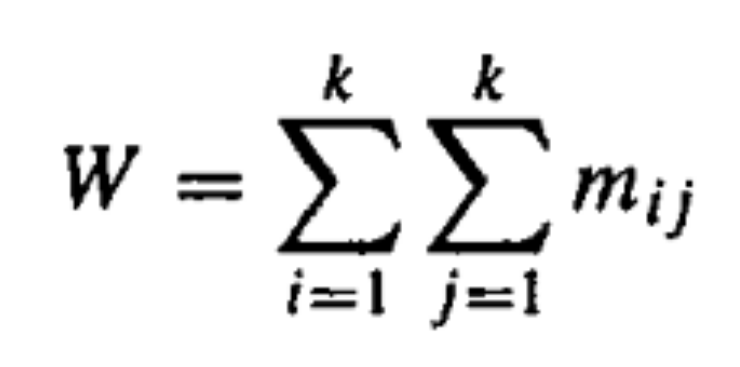
\includegraphics[width=0.25\textwidth]{imagenes/wsum} 
	\caption{Definición de W \cite{ref14}}
\end{figure}

Sabemos que, como mucho, ($k^2$ - k) entradas de M pueden ser etiquetadas como no monotónicas, por tanto el índice de no-monotonicidad queda así:

\begin{figure}[H]
	\centering
	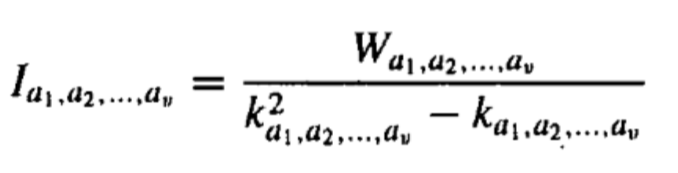
\includegraphics[width=0.5\textwidth]{imagenes/inm} 
	\caption{Definición índice de no-monotonicidad \cite{ref14}}
\end{figure}

Previo cálculo del índice que nos dirá como de bueno es un árbol tanto en precisión como en aguardar las restricciones monotónicas, calculamos el \textbf{order-ambiguity-score}, que se define en términos del índice previamente calculado tal como sigue:

\begin{figure}[H]
	\centering
	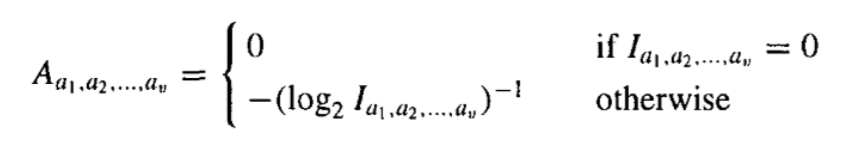
\includegraphics[width=0.75\textwidth]{imagenes/oas} 
	\caption{Definición de order-ambiguity-score \cite{ref14}}
\end{figure}

Finalmente, añadimos esta medida de no-monotonicidad calculada a nuestra medida de precisión E-score de la siguiente manera:

\begin{figure}[H]
	\centering
	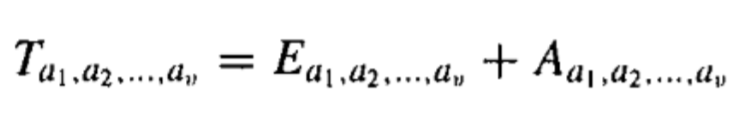
\includegraphics[width=0.55\textwidth]{imagenes/tas} 
	\caption{Definición de total-ambiguity-score \cite{ref14}}
\end{figure}

Una vez tenemos creada la métrica, ya sabemos que, a menor valor, mejor será el resultado, ya que significará que poseemos un menor fallo en la predicción y una mayor conservación de las relaciones de montonía dentro del árbol.

Esta forma de evaluar un árbol de decisión no implica que las consideraciones de monotonía deban dominar la construcción del árbol necesariamente. Podemos decidir cuánta importancia darle al proceso de construcción de un árbol montónico multiplicando el order-ambiguity-score por un factor para darle menor importancia al hecho de que el árbol aguarde las restricciones monotónicas con respecto al de que consiga una buena precisión en la predicción. \cite{ref14}

\newpage



\chapter[Capítulo 4. Propuesta]{Propuesta}

\section{Introducción}

Una vez conocemos el funcionamiento, características, algunas formas de implementación y los problemas a los que se enfrentan cada una de las técnicas descritas hasta ahora (es decir, de los árboles de decisión, el data streaming y la aplicación de restricciones monotónicas), procedemos a exponer la propuesta hacia la cual se encauza el propósito de este documento.\\

Hemos comprobado que existen métodos eficientes de adquisición de conocimiento y predicción sobre flujos de datos utilizando árboles de decisión, tales como Option trees y Hoeffding Anytime Tree (HATT), ambos basados en Hoeffding Tree, o incluso su versión mejorada para la detección del cambio de concepto en el tiempo (CVFDT).\\

Así mismo, hemos observado también que existen ejemplos de conjuntos de datos que poseen características dignas de ser tenidas en cuenta a la hora de crear un modelo de aprendizaje de conocimiento, ya que aportan una base de información subyacente a los datos que ofrece al algoritmo la capacidad de crear una estructura de datos más eficiente para la resolución de cualquier problema que se enfrente a datos de este estilo. Evidentemente hablamos de los conjuntos de datos que aguardan en sí una relación de monotonía entre los valores de los atributos de sus instancias y las clases asignadas a estas.\\

Tal como se muestra en \cite{ref14}, existen multitud de problemas en la vida diaria que requieren ser tratados como problemas de clasificación monotónica con el fin de ser correctamente resueltos. Este es el caso de aquella universidad que no quiera admitir a un solicitante con ciertas notas y rechazar a otro con notas iguales o más altas por no haber tenido en cuenta la monotonicidad del asunto, o el caso de una compañía de seguros de vida que no desea que sus decisiones dependan de un árbol de decisión que no tenga en cuenta que un solicitante anciano y poco saludable ha de cotizar una tasa de prima más alta que un solicitante joven y saludable. Otros problemas pueden ser los de credit scoring, elección de consumidor, selección de escuela y transporte, etc.\\

En el siguiente ejemplo veremos las consecuencias que puede tener el hecho de crear un árbol de clasificación no-monotónico en un problema de credit scoring simple. Los atributos utilizados en cada árbol son los activos + los ingresos y los activos a solas respectivamente. 


\begin{figure}[H]
	\centering
	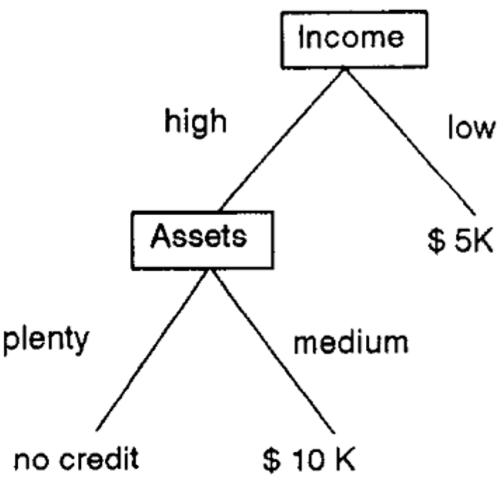
\includegraphics[width=1\textwidth]{imagenes/ejAr} 
	\caption{Árboles no monotónicos\cite{ref14}}
\end{figure}

Como vemos, ambos árboles, al no poseer restricciones de monotonicidad, carecen también de sentido, ya que a un cliente con pocos activos se le autoriza una linea de crédito de cinco mil dólares, mientras que a un cliente con más activos no se le ofrece crédito alguno, por ejemplo.

A la derecha podemos observar el árbol resultante aplicado a un conjunto de datos que \textbf{sí} guarda relación de monotonía entre los valores de los atributos y las clases asignadas y que, tal como vemos, no asegura que el árbol creado a partir de él sea monotónico.\\
Los datos utilizados para ello son los siguientes:

\begin{figure}[H]
	\centering
	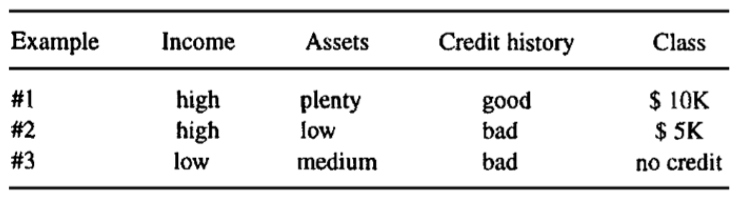
\includegraphics[width=0.9\textwidth]{imagenes/tablaEj} 
	\caption{Conjunto de datos monotónico\cite{ref14}}
\end{figure}

\section{Propuesta y resultados esperados}

Visto todo esto, parece lógico crear una adaptación de los algoritmos de árboles de decisión para data streaming que además posean información sobre restricciones de monotonía para conseguir resultados superiores en cuanto al análisis del dominio del problema al que se enfrentan los algoritmos que trabajan con este tipo de conjuntos de datos.\\

La propuesta no pretende conseguir resultados mejores en cuanto al accuracy obtenido en la predicción de resultados si no que, pretende que las estructuras creadas por los árboles de decisión para flujos de datos sean más fieles a la realidad que subyace bajo data sets con cierto nivel de monotonía en su relación atributos-clase.\\

Dicho esto, podría darse el caso en el que el algoritmo básico comparativo sin restricciones de monotonía alcance un accuracy superior al que puedan alcanzar las adaptaciones realizadas las cuales si posean información sobre dichas relaciones monotónicas.\\

\section{Algoritmos a comparar}

Como \textbf{algoritmo de comparación} utilizaremos aquél del cual la literatura ha hecho más uso para la realización de estudios comparativos y mejoras de otros aspectos, es decir: \textbf{Hoeffding Tree}, la base de la que parten gran cantidad de algoritmos de árboles de decisión para el tratamiento de data streaming.\\

Los \textbf{algoritmos que pretenden hacerle frente} en cuanto a los aspectos ya mencionados serán:
\begin{itemize}
	\item Adaptación de Hoeffding Tree con restricciones monotónicas mediante el uso del \textbf{método basado en matriz}.
	\item Adaptación de Hoeffding Tree con restricciones monotónicas mediante el uso del \textbf{método de evaluación de monotonicidad de ramas}.
	\item Adaptación de Hoeffding Tree con restricciones monotónicas mediante el uso de\textbf{ ambos métodos al mismo tiempo}.
\end{itemize}











\newpage



\chapter[Capítulo 5. Software desarrollado y uso]{Software desarrollado y uso}

El software para la realización de los experimentos ha sido creado mediante el IDE de programación Netbeans con Java como lenguaje de programación.

Los datos empleados son estáticos, por lo que ha sido necesario adaptar el código fuente a un entorno de flujo de datos para poder realizar los experimentos.

Como ya se ha comentado, el algoritmo de partida de los experimentos es el Hoeffding Tree, el cual se basa en una adaptación de árboles de decisión para flujos de datos. Este código ha sido tomado de la API de MOA.

MOA (Massive Online Analisys) \cite{ref31} es un entorno de trabajo open-source relacionado con el proyecto WEKA (Waikato Environment for Knowledge Analysis) para el tratamiento o minería de flujos de datos de evolución masiva conteniendo una gran colección de algoritmos de machine
learning como son: clasificación, regresión, clustering, detección de outliers, detección de concept drift y sistemas de recomendación, así como herramientas de evaluación. 

Los \textbf{algoritmos implementados} son los descritos en la propuesta:
\begin{itemize}
	\item Algoritmo 1: Árboles de clasificación monotónica sobre flujos de datos. Método de matriz de colisiones.
	\item Algoritmo 2: Árboles de clasificación monotónica sobre flujos de datos. Método de evaluación a la hora de expandir el árbol.
\end{itemize}

Para la obtención de resultados y la posible comparativa de estos entre los distintos modelos, para ambos algoritmos ha sido necesario modificar algunos de los parámetros de Hoeffding Tree:
\begin{itemize}
	\item \textbf{Desempate(tie-breaking)}: este parámetro ayuda, tal como su propio nombre indica, a evitar estancamientos en las expansiones de los árboles acaecidos por la similitud entre la ganancia ofrecida por dos atributos a la hora de decidirse por alguno para expandir. Si son muy similares, la diferencia entre ellos sera pequeña, por tanto será imposible que supere la cota Hoeffding, lo cual es necesario para poder expandir. Gracias a su modificación, he podido obtener árboles más extensos, ya que sin tocarlo, el pequeño volumen de datos manejado no lo permitía.
	\item \textbf{Grace period option}: con él indicamos la cantidad de instancias necesarias para la generación de nodos nuevos en el árbol.
\end{itemize}

Dichos han sido creados adaptando el código y resultados de Hoeffding Tree a las necesidades de cada uno y, los resultados de estos han sido sometidos a\textbf{ validación cruzada de 10 iteraciones} para obtener resultados más fieles al comportamiento de cada algoritmo. Para obtener los resultados de cada iteración de la validación cruzada he creado mis propias\textbf{ funciones de evaluación} de la medida de \textbf{accuracy (MAE en este caso)} y del \textbf{índice de no-monotonicidad (NMI).}

\textbf{Para la obtención de} la medida \textbf{MAE}, como ya hemos visto, simplemente divido la suma de errores de cada iteración entre la cantidad de elementos en el conjuntos de datos. 

\textbf{Para obtener el NMI} hago uso de los datos predichos por el algoritmo de la siguiente forma:
\begin{enumerate}
	\item Detecto las colisiones entre las distintas instancias (es decir, compruebo con cuantas instancias no aguarda monotonía respecto a atributos y clase cada una de las instancias del conjunto de datos).
	\item Realizo la suma de dichas colisiones.
	\item Dividio entre la cantidad máxima de colisiones que podrían ocurrir en dicho conjunto de datos.
\end{enumerate}

El \textbf{proceso de aprendizaje del modelo y validación del mismo} para cada iteración de la validación cruzada es el siguiente:
\begin{enumerate}
	\item Entrenamiento del modelo con el algoritmo escogido de los tres implementados haciendo uso de los datos de entrenamiento a modo de flujo de datos.
	\item Generación de predicciones con los datos de test.
	\item Validación de las predicciones en cuanto a accuracy (MAE) y monotonicidad (NMI).
\end{enumerate}

Estos resultados obtenidos son los que se expondrán más adelante en la comparativa de algoritmos.

\newpage



\chapter[Capítulo 6. Experimentos]{Experimentos}

Tras el análisis introductorio al contexto en el que nos situamos para hacer conocer al lector las técnicas que hay detrás del problema que queremos resolver y después de exponer y analizar la propuesta de trabajo a la que nos enfrentamos, entramos de lleno en la exposición del marco de trabajo en el que nos situaremos con los algoritmos que vamos a manejar, así como la muestra de resultados obtenidos en cuanto a comparativas realizadas y, por último, su posterior análisis, con el fin de concretar el éxito o fracaso de la teoría expuesta en capítulos anteriores.

\section{Marco de trabajo}

En esta sección, tal como hemos comentado, situaremos el marco de trabajo de nuestro experimento, formado por los conjuntos de datos que trataremos para este, junto con las medidas de precisión y monotonía que usaremos con los algoritmos con el fin de poder ser comparados por igual.

\subsection{Conjuntos de datos}

Primeramente comentaremos los conjuntos de datos a tratar con el fin de entender a que se enfrentarán nuestros algoritmos. Antes que nada cabe destacar que los data sets que vamos a utilizar son estáticos, es decir, no son datos que nos llegan en flujo (que es uno de los aspectos que queremos tratar en este documento), por tanto a la hora de realizar los experimentos habremos de simular la entrada de datos por un flujo en lugar de leerlos de forma directa. Los datos han sido sacados de \cite{ref16}



\begin{table}[]
	\begin{tabular}{|l|l|l|l|l|l|l|}
		\hline
		Data set & Instancias & Atributos & Numéricos & Nominales & Clases & NMI   \\ \hline
		ERA      & 1000       & 4         & 4         & 0         & 9      & 0.016 \\ \hline
		ESL      & 488        & 4         & 4         & 0         & 9      & 0.004 \\ \hline
		LEV      & 1000       & 4         & 4         & 0         & 5      & 0.006 \\ \hline
		SWD      & 1000       & 10        & 10        & 0         & 4      & 0.009 \\ \hline
	\end{tabular}
	\caption{Conjuntos de datos a utilizar en el experimento}
\end{table}

\subsubsection{Descripción de los conjuntos de datos}

\begin{itemize}
	\item \textbf{ERA}: recopilación de datos tomados durante un experimento académico de toma de decisiones académicas con el objetivo de determinar las cualidades más importantes  de los candidatos para ciertos tipos de trabajo.
	\item \textbf{ESL}: perfiles de aplicantes para ciertos trabajos en la industria. Psicólogos expertos determinaron los valores de los atributos de los datos basándose en resultados de tests psicométricos y entrevistas realizadas a los candidatos.
	\item \textbf{LEV}: estos datos hacen referencia a ejemplos de evaluaciones anónimas de profesores realizadas al final de cursos MBA (Master of Business Administration). Antes de recibir las notas finales, se le pidió a los estudiantes que puntuaran a sus profesores en concordancia a cuatro atributos como las habilidades orales y la contribución a su conocimiento profesional o general. La salida es una evaluación total del rendimiento del profesor.
	\item \textbf{SWD}: este conjunto de datos contiene evaluaciones reales de trabajadores sociales cualificados midiendo el riesgo de un grupo de niños al permanecer en casa con sus familias. Esta evaluación de riesgos se presenta a menudo en cortes judiciales para ayudar a decidir que le interesa más a un niño presuntamente maltratado o descuidado.
\end{itemize}



\subsection{Medidas}

Primeramente abordaremos las medidas destinadas a valorar la precisión y, posteriormente, aquellas cuyo objetivo es medir la monotonicidad \cite{ref15}.

\subsubsection{Medidas de precisión}

Dentro de las medidas de precisión para clasificación podemos encontrarlas de dos tipos: para clasificación binaria y para clasificación multiclase.

\textbf{Clasificación binaria}

Previa exposición de algunos de las medidas de clasificación binaria necesitamos tener en cuenta algunos términos con el fin de poder entenderlas:
\begin{itemize}
	\item \textbf{True Positives (TP)}: cantidad de instancias con predicción positiva que están correctamente clasificadas.
	\item \textbf{False Positives (FP)}: cantidad de instancias con predicción positiva que no están correctamente clasificadas.
	\item \textbf{True Negative (TN)}: cantidad de instancias con predicción negativa que están correctamente clasificadas.
	\item \textbf{False Negative (FN)}: cantidad de instancias con predicción negativa que no están correctamente clasificadas.
\end{itemize}

Una vez conocemos esta terminología, vemos algunas de las medidas para clasificación binaria:

\begin{itemize}
	\item \textbf{Accuracy}: Representa la habilidad predictiva de acuerdo con la proporción de 
	los datos clasificados de forma correcta.
	\begin{figure}[H]
		\centering
		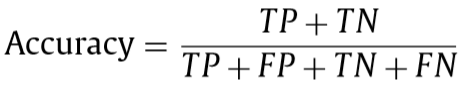
\includegraphics[width=0.5\textwidth]{imagenes/f2} 
	\end{figure}

	\item \textbf{Error rate}: Caso opuesto al accuracy, evaluando la proporción de los datos
	evaluados clasificados de forma incorrecta.
	\begin{figure}[H]
		\centering
		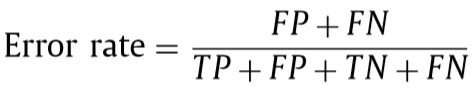
\includegraphics[width=0.5\textwidth]{imagenes/f3} 
	\end{figure}

	\item \textbf{Recall/sensitivity}: Medida de la proporción de TP que están correctamente clasificados.
	\begin{figure}[H]
		\centering
		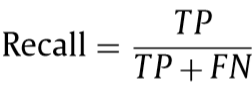
\includegraphics[width=0.3\textwidth]{imagenes/f4} 
	\end{figure}

	\item \textbf{Positive predictive value(PPV)/Precisión}: Proporción de las instancias del test que tienen una
	salida positiva y que además están bien clasificados.
	representa la probabilidad de que una prueba positiva 
	refleje la condición subyacente que se está probando.
	\begin{figure}[H]
		\centering
		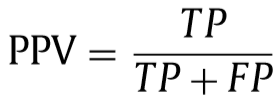
\includegraphics[width=0.3\textwidth]{imagenes/f5} 
	\end{figure}
\end{itemize}



\textbf{Clasificación multiclase}

Procedemos ahora a exponer algunas medidas de predicción aplicadas a los problemas de clasificación multiclase. Para ambas medidas hemos de tener en cuenta lo siguiente: n corresponde a la cantidad de observaciones en el conjunto de datos evaluados, $y'_i$ es la clase predicha para una instancia i e $y_i$ es la etiqueta de clase real (ambos representados como valores enteros basados en su posición en la escala ordinal).

\begin{itemize}
	\item \textbf{Mean Squared Error (MSE)}: Mide la media de los cuadrados de los errores. Al usar los cuadrados de $y_i$ e $y'_i$ se pondera con un peso mayor a los errores más grandes.
	\begin{figure}[H]
		\centering
		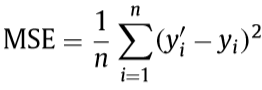
\includegraphics[width=0.4\textwidth]{imagenes/f6} 
	\end{figure}

	\item \textbf{Mean Absolute Error (MAE)}: Mide cómo de cerca se encuentran las predicciones de los valores reales de salida. MAE es una medida lineal, lo que significa que los errores son tratados con el mismo peso en la media.
	\begin{figure}[H]
		\centering
		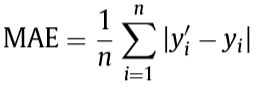
\includegraphics[width=0.4\textwidth]{imagenes/f7} 
	\end{figure}
\end{itemize}

Dados los conjuntos de datos de los que disponemos y el uso que la literatura recomienda hacer de las medidas de precisión sobre este tipo de conjuntos de datos, utilizaremos la medida\textbf{ Mean Absolute Error (MAE)} para la evaluación de la precisión de nuestros algoritmos, ya que los conjuntos que manejaremos son de clasificación multiclase.

\subsubsection{Medidas de monotonicidad}

Nuestro propósito con esta medida es evaluar la tasa de monotonicidad provista tanto por las predicciones obtenidas y el conjunto de datos original, como de la construcción del modelo.

Para ello tenemos en cuenta las siguientes consideraciones:
\begin{itemize}
	\item x es un ejemplo del conjunto de datos D.
	\item NClash(x) es la cantidad de ejemplos de D que no cumplen las restricciones de monotonicidad con respecto a x.
	\item n es el número de instancias en D.
	\item NMonot(x) es el número de ejemplos de D que sí que cumplen las restricciones de monotonicidad con respecto a x.
\end{itemize}

El \textbf{Índice de no-monotonicidad} se define como el número de choques (Nclash) dividido por el número de pares de ejemplos en el conjunto de datos:

\begin{figure}[H]
	\centering
	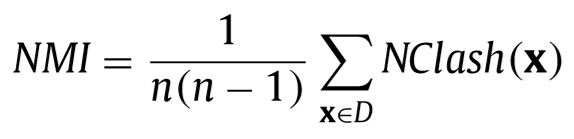
\includegraphics[width=0.5\textwidth]{imagenes/f8} 
\end{figure}

Y esta será la medida que utilicemos finalmente para la evaluación de la monotonicidad en nuestros algoritmos.

\section{Resultados}

A continuación muestro las condiciones bajo las que se han ejecutado todas las tablas de resultados que mostraré a continuación. Estas condiciones son los parámetros de Hoeffding Tree ajustados para obtener un árboles lo suficientemente representativos de los datos.
\begin{itemize}
	\item Parámetro de desempate: 1
	\item Parámetro grace period:
	\begin{itemize}
		\item ERA = 20
		\item ESL = 45
		\item LEV = 20
		\item SWD = 20
	\end{itemize}
\end{itemize}

Como era de esperar, el conjunto de datos ESL, al ser bastante más pequeño que los demás, necesita un aumento del parámetro grace period.

Para el segundo algoritmo, el que trata los índices de monotonicidad de los nodos para decidir si hacer una expansión de este o no, posee además un parámetro de tolerancia de no-monotonicidad para evitar intentar conseguir árboles muy monótonos a costa de la pérdida de precisión. El parámetro es un simple factor del NMI calculado en cada nodo con respecto a las demás ramas. Los ajustes de este parámetro para los experimentos han sido calculados de forma empírica hasta obtener unos resultados óptimos. Estos son:
\begin{itemize}
	\item ERA = 0.5
	\item ESL = 0.45
	\item LEV = 1
	\item SWD = 0.45
\end{itemize}

\begin{table}[H]
	\begin{tabular}{|c|l|l|l|l|}
		\hline
		HF & ERA    & ESL    & LEV &  SWD \\ \hline
		MAE & 1.673 & 0.580 & 0.612                      & 0.625                     \\ \hline
		NMI & 0.4060 & 0.3856 & 0.3473                     & 0.3510                     \\ \hline
	\end{tabular}
\caption{Resultados de accuracy y monotonicidad para los 4 data sets descritos mediante el uso de Hoeffding Tree algorithm.}
\end{table}

\begin{table}[H]
	\begin{tabular}{|c|l|l|l|l|}
		\hline
		HF + Poda & ERA    & ESL    & LEV &  SWD \\ \hline
		MAE & 1.88 & 0.576 & 0.636                      & 0.66                     \\ \hline
		NMI & 0.3892 & 0.3849 & 0.3382                     & 0.342                     \\ \hline
	\end{tabular}
	\caption{Resultados de accuracy y monotonicidad para los 4 data sets descritos mediante el uso de Hoeffding Tree algorithm junto con poda.}
\end{table}

\begin{table}[H]
	\begin{tabular}{|c|l|l|l|l|}
		\hline
		HF + Decisión & ERA    & ESL    & LEV &  SWD \\ \hline
		MAE & 1.65 & 0.642 & 0.562                      & 0.62                     \\ \hline
		NMI & 0.3957 & 0.3791 & 0.3369                     & 0.3458                     \\ \hline
	\end{tabular}
	\caption{Resultados de accuracy y monotonicidad para los 4 data sets descritos mediante el uso de Hoeffding Tree algorithm junto con el algoritmo de toma de decisión a la hora de expandir.}
\end{table}

\begin{table}[H]
	\begin{tabular}{|c|l|l|l|l|}
		\hline
		HF + Poda + Decisión & ERA    & ESL    & LEV &  SWD \\ \hline
		MAE & 1.67 & 0.64 & 0.664                      & 0.629                     \\ \hline
		NMI & 0.3815 & 0.3790 & 0.3451                     & 0.3447                     \\ \hline
	\end{tabular}
	\caption{Resultados de accuracy y monotonicidad para los 4 data sets descritos mediante el uso de Hoeffding Tree algorithm junto con ambos algoritmos creados.}
\end{table}
\newpage

\section{Análisis}

A la vista de los resultados podemos observar que, aunque no en gran medida, la adición de restricciones monotónicas a los algoritmos de flujos de datos con árboles de decisión resulta ser exitosa, ya que el índice de no-monotonicidad desciende al aplicar cualquiera de los algoritmos creados, ya sea el de poda, el de toma de decisión a la hora de expandir los nodos o ambos al mismo tiempo.\\

Hemos de tener en cuenta también que los conjuntos de datos que estamos tratando en los experimentos son muy pequeños, el entorno de flujos de datos real ofrece cantidades masivas de datos que permiten a los algoritmos un aprendizaje más fiel del problema, quizá este sea el motivo de que el índice de monotonicidad descienda tan poco entre el algoritmo sin las restricciones y los que sí las tienen. Al no tener tantos datos hemos debido de modificar los parámetros de Hoeffding Tree para poder crear árboles lo suficientemente grandes que nos sirvan para poder probar nuestros algoritmos.\\

Por contra, podemos observar cómo en algunas ocasiones, un descenso de la monotonicidad viene acarreado de sanciones en la precisión del algoritmo, por lo que el índice MAE puede verse ligeramente mayor a la hora de aplicar estas restricciones monotónicas. Como dijimos capítulos atrás, el objetivo del presente documento era la disminución de la monotonicidad de los resultados predichos por nuestros algoritmos. Es probable que el algoritmo base, sin las restricciones de monotonía, alcance una precisión más alta pero que la interpretabilidad de los resultados predichos sea inferior a la de los resultados obtenidos por los algoritmos que sí aplican dichas restricciones.\\

En definitiva, teniendo en cuenta que el factor que hace que los resultados no sean tan significativos es el volumen de los conjuntos de datos tratado, podemos concluir que los resultados han sido exitosos ya que, aunque hemos obtenido mayor error en la predicción, la interpretabilidad de los resultados es mayor debido a la bajada de la no-monotonicidad en las predicciones.

\newpage












\chapter[Capítulo 7. Conclusiones y trabajo futuro]{Conclusiones y trabajo futuro}

Finalmente, una vez explicado el desarrollo completo del proyecto, es el momento de mirar hacia atrás para cerciorarme de las asignaturas del grado cursadas sin las que no hubiera sido capaz de desenvolverme de manera tan efectiva para la realización del proyecto, así como darme cuenta de los conocimientos que he adquirido durante esta etapa de mi carrera y, por último, realizar una valoración de todo ello.


\newpage












%
%
%%\nocite{*}
\bibliography{citas} %archivo citas.bib que contiene las entradas 
\bibliographystyle{plain} % hay varias formas de citar

%\input{capitulos/Anexo}

%
%\appendix
%\input{apendices/manual_usuario/manual_usuario}
%%\input{apendices/paper/paper}
%\input{glosario/entradas_glosario}
% \addcontentsline{toc}{chapter}{Glosario}
% \printglossary
\chapter*{}
\thispagestyle{empty}

\end{document}
